% Saberes básicos (LOMLOE) asociados a esta unidad
%
% B. La materia
%   - Teoría cinético-molecular: aplicación a observaciones sobre la materia explicando
%     sus propiedades, los estados de agregación y los cambios de estado. Es el eje
%     central de la unidad: toda la unidad explica los estados de agregación (sólido,
%     líquido, gas) y los cambios de estado (fusión, ebullición, evaporación,
%     sublimación...) a partir del modelo de partículas en movimiento.
%   - Experimentos relacionados con los sistemas materiales: conocimiento y descripción
%     de sus propiedades. Se describen propiedades como la compresibilidad, la
%     densidad relativa de los estados o la presión de un gas, ligadas al
%     comportamiento de las partículas.
%
% C. La energía
%   - Efectos del calor sobre la materia: análisis de los efectos y aplicación en
%     situaciones cotidianas. Se estudia cómo el calor produce cambios de estado, la
%     curva de calentamiento/enfriamiento y el concepto de calor latente, así como
%     fenómenos cotidianos (niebla, rocío, olla a presión, altitud y ebullición...).
%
% A. Las destrezas científicas básicas
%   - El lenguaje científico: unidades del Sistema Internacional. Se usan
%     sistemáticamente unidades de presión, volumen y temperatura (atmósferas, litros,
%     kelvin) y el manejo de \qty{}{} de siunitx en los ejemplos y ejercicios numéricos
%     de las leyes de los gases.
%   - Estrategias de interpretación y producción de información científica. Se
%     interpretan tablas de puntos de fusión/ebullición y gráficas de calentamiento
%     descritas verbalmente para extraer conclusiones.

\spacing{1.3}
\raggedbottom % pages with large figures end where the text ends (no stretched gaps between boxes)

\section{Physical states of matter}

On the Earth, almost everything around us is a \textbf{solid}, a \textbf{liquid} or a \textbf{gas}. Each state has its own ``personality'':

\begin{figure}[H]
    \centering
    % [FIGURA ORIGINAL] \includegraphics[width=\textwidth]{Unit_2/states_overview}
    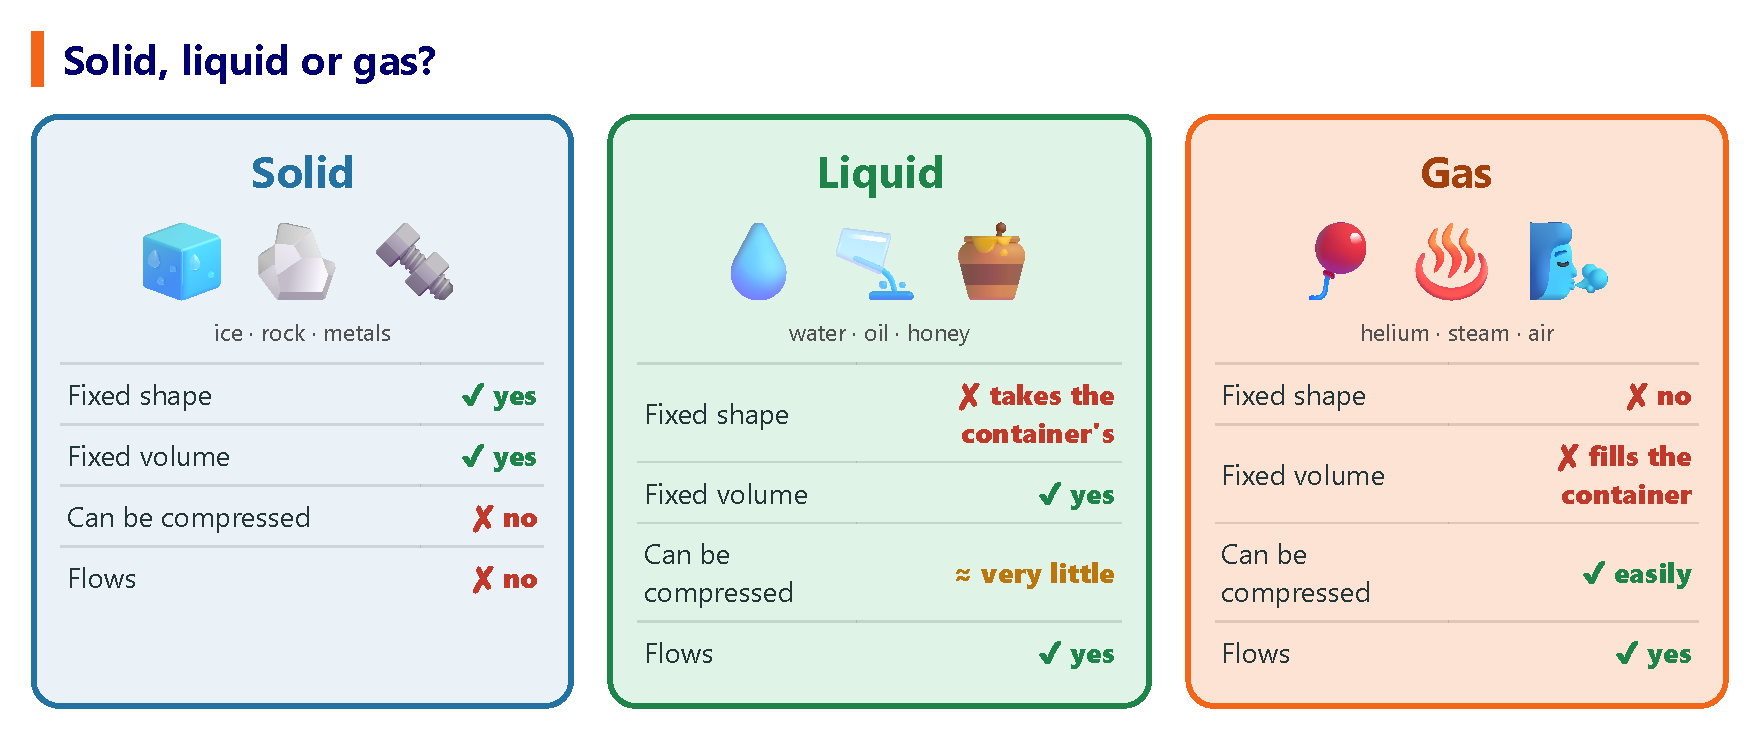
\includegraphics[width=\textwidth]{FigurasSVG/Unit_2_State_of_Matter/pdf/states_overview.pdf}
    \caption{The properties of solids, liquids and gases.}
    \label{fig:u2_states_overview}
\end{figure}

\subsection{Plasma: the fourth state of matter}

Solid, liquid and gas are not the only states of matter. There is a \negsubro{fourth state}, called \textbf{plasma}.

\begin{definition}[Plasma]
    A gas that is so \textbf{hot} that its particles break and become \textbf{electrically charged}. That is why a plasma \textbf{glows} (gives out light) and conducts electricity. It is considered the \textbf{fourth state of matter}.
\end{definition}

\begin{figure}[H]
    \centering
    % [FIGURA ORIGINAL] \includegraphics[width=\textwidth]{Unit_2/plasma}
    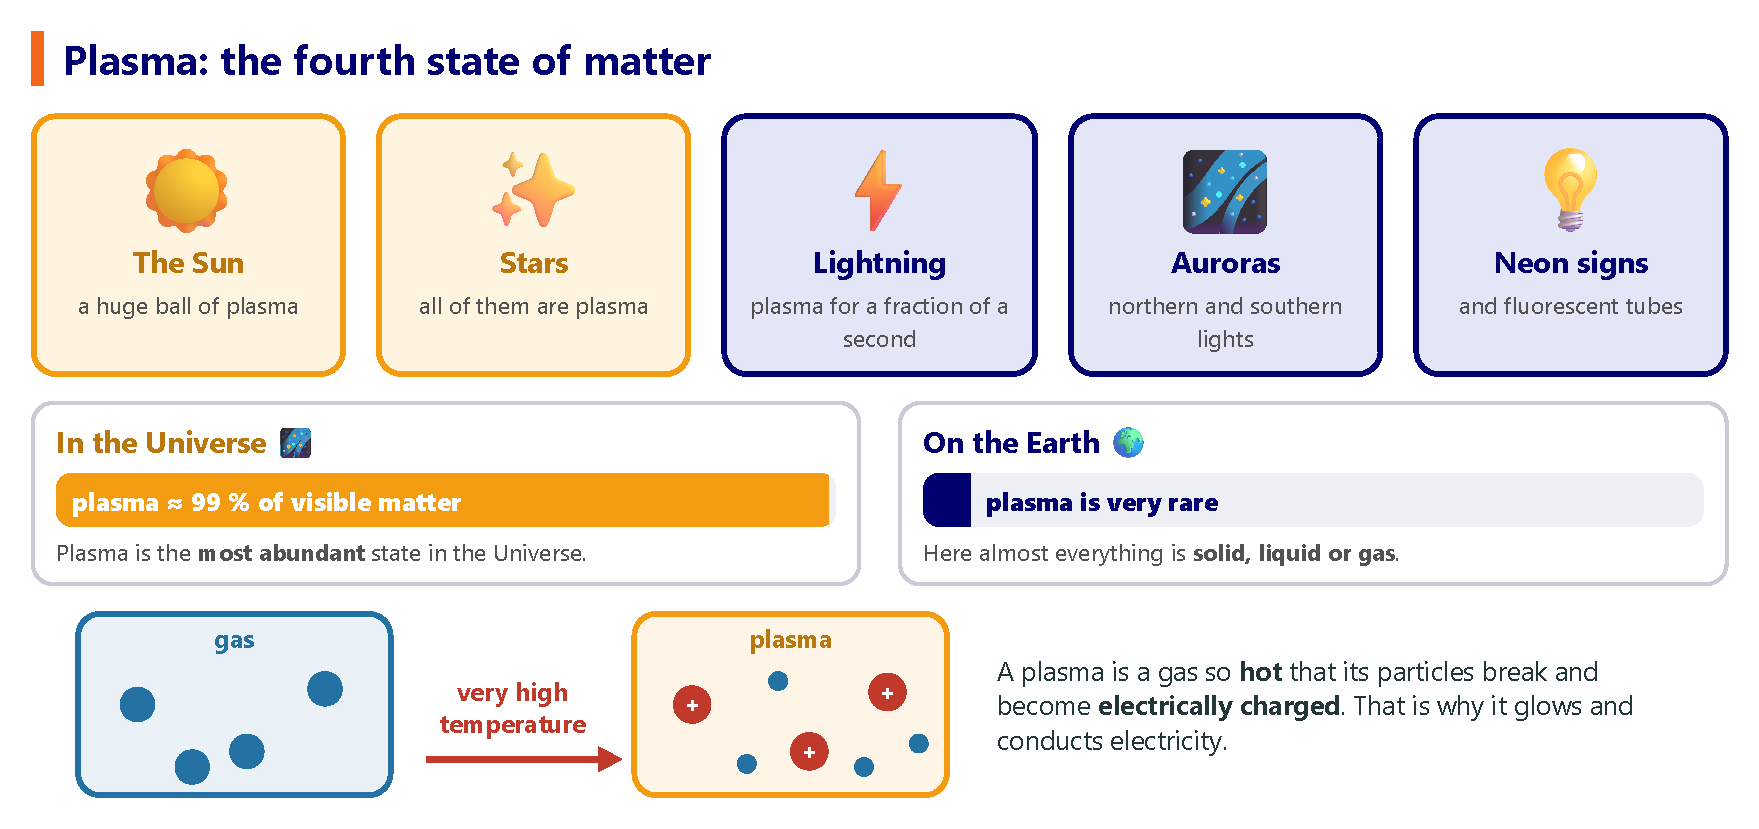
\includegraphics[width=\textwidth]{FigurasSVG/Unit_2_State_of_Matter/pdf/plasma.pdf}
    \caption{Plasma is the most abundant state in the Universe, but it is very rare on the Earth.}
    \label{fig:u2_plasma}
\end{figure}

\begin{impt}
    \begin{itemize}
        \item Plasma is the \textbf{most abundant} state of matter \textbf{in the Universe}: the \textbf{Sun} and all the stars are huge balls of plasma.
        \item On the \textbf{Earth}, however, plasma is \textbf{very rare}: we only see it in lightning, in the auroras (northern lights) and in neon signs and fluorescent tubes.
    \end{itemize}
\end{impt}

\begin{didyouknow}
    There are also \textbf{liquid crystals}, a strange state between a liquid and a solid. They are used in the LCD screens of mobile phones and televisions.
\end{didyouknow}

\begin{exercise}
    Classify each substance as a solid, a liquid or a gas at room temperature: wood, natural gas, oil, water, aluminium, oxygen, alcohol, carbon dioxide, sand.
    \begin{solu}
        \textbf{Solids}: wood, aluminium, sand. \\
        \textbf{Liquids}: oil, water, alcohol. \\
        \textbf{Gases}: natural gas, oxygen, carbon dioxide.
    \end{solu}
\end{exercise}

\begin{exercise}
    Answer these questions about plasma:
    \begin{enumerate}[label=\letraminuscula]
        \item Why is plasma called the ``fourth state of matter''?
        \item Which is the most abundant state of matter in the Universe? And on the Earth?
        \item Give two examples of plasma that you can see on the Earth.
    \end{enumerate}
    \begin{solu}
        \begin{enumerate}[label=\alph*)]
            \item Because it is different from solids, liquids and gases: it is a gas so hot that its particles are electrically charged.
            \item In the Universe, plasma (the Sun and the stars). On the Earth, plasma is very rare: most matter is solid, liquid or gas.
            \item Lightning, auroras, neon signs, fluorescent tubes.
        \end{enumerate}
    \end{solu}
\end{exercise}

\begin{exercise}
    Decide whether each statement is true or false, and correct the false ones.
    \begin{enumerate}[label=\letraminuscula]
        \item Sand flows, so it is a liquid.
        \item A sponge can be compressed, so it is a gas.
        \item The sponge is made of a porous, flexible material with air inside, so it can be compressed.
    \end{enumerate}
    \begin{solu}
        \begin{enumerate}[label=\alph*)]
            \item \textbf{False}. Sand is a solid made up of very small grains that seem to behave like a liquid, but each grain keeps its own shape and size.
            \item \textbf{False}. A sponge is a solid; it is compressible because it is porous (it has air inside), not because it is a gas.
            \item \textbf{True}.
        \end{enumerate}
    \end{solu}
\end{exercise}

\begin{exercise}
    A student has three identical closed syringes: syringe A contains air, syringe B contains water, and syringe C contains a small metal ball. The student blocks the tip of each syringe and pushes the plunger as hard as possible.
    \begin{enumerate}[label=\letraminuscula]
        \item In which syringe can the plunger be pushed in noticeably?
        \item Explain the result in terms of the compressibility of solids, liquids and gases.
    \end{enumerate}
    \begin{solu}
        \begin{enumerate}[label=\alph*)]
            \item Only in \textbf{syringe A} (the one with air).
            \item Gases can be compressed because there is a lot of empty space between their particles. Liquids (syringe B) and solids (syringe C) cannot be compressed, since their particles are already almost touching.
        \end{enumerate}
    \end{solu}
\end{exercise}

%----------------------------------------------------------------------------------------

\section{Kinetic theory and states of matter}

Why is ice hard, water runny and steam invisible, if all three are the same substance? To answer this question, scientists imagine matter as if it were made of tiny ``balls''. This idea is called the \negsubro{kinetic theory} (``kinetic'' comes from a Greek word that means ``movement'').

\begin{definition}[Kinetic theory]
    A scientific model that explains how matter behaves by imagining that it is made of tiny \textbf{particles} that are \textbf{always moving}.
\end{definition}

The kinetic theory can be summed up in four simple ideas:

\begin{enumerate}[label=\numberballmDarkTeal]
    \item \textbf{Everything is made of particles.} All matter is made of tiny particles, so small that we cannot see them, not even with a normal microscope.
    \item \textbf{The particles never stop moving.} They vibrate, move around and bump into each other all the time.
    \item \textbf{Hotter means faster.} When we heat a substance, its particles move faster; when we cool it, they move more slowly. \textbf{Temperature} tells us how fast the particles are moving.
    \item \textbf{The particles attract each other.} They are held together by forces, like invisible ``glue''. How strong this glue is, compared with how fast the particles move, decides whether the substance is a \textbf{solid}, a \textbf{liquid} or a \textbf{gas}.
\end{enumerate}

\begin{impt}
    Think of the pupils in your school: in class they are sitting in their places and only fidget a little (\textbf{solid}); in the corridor they walk and move past each other, but stay close together (\textbf{liquid}); in the playground they run freely in all directions, far from each other (\textbf{gas}).
\end{impt}

\begin{figure}[H]
    \centering
    % [FIGURA ORIGINAL] \includegraphics[width=\textwidth]{Unit_2/particle_model}
    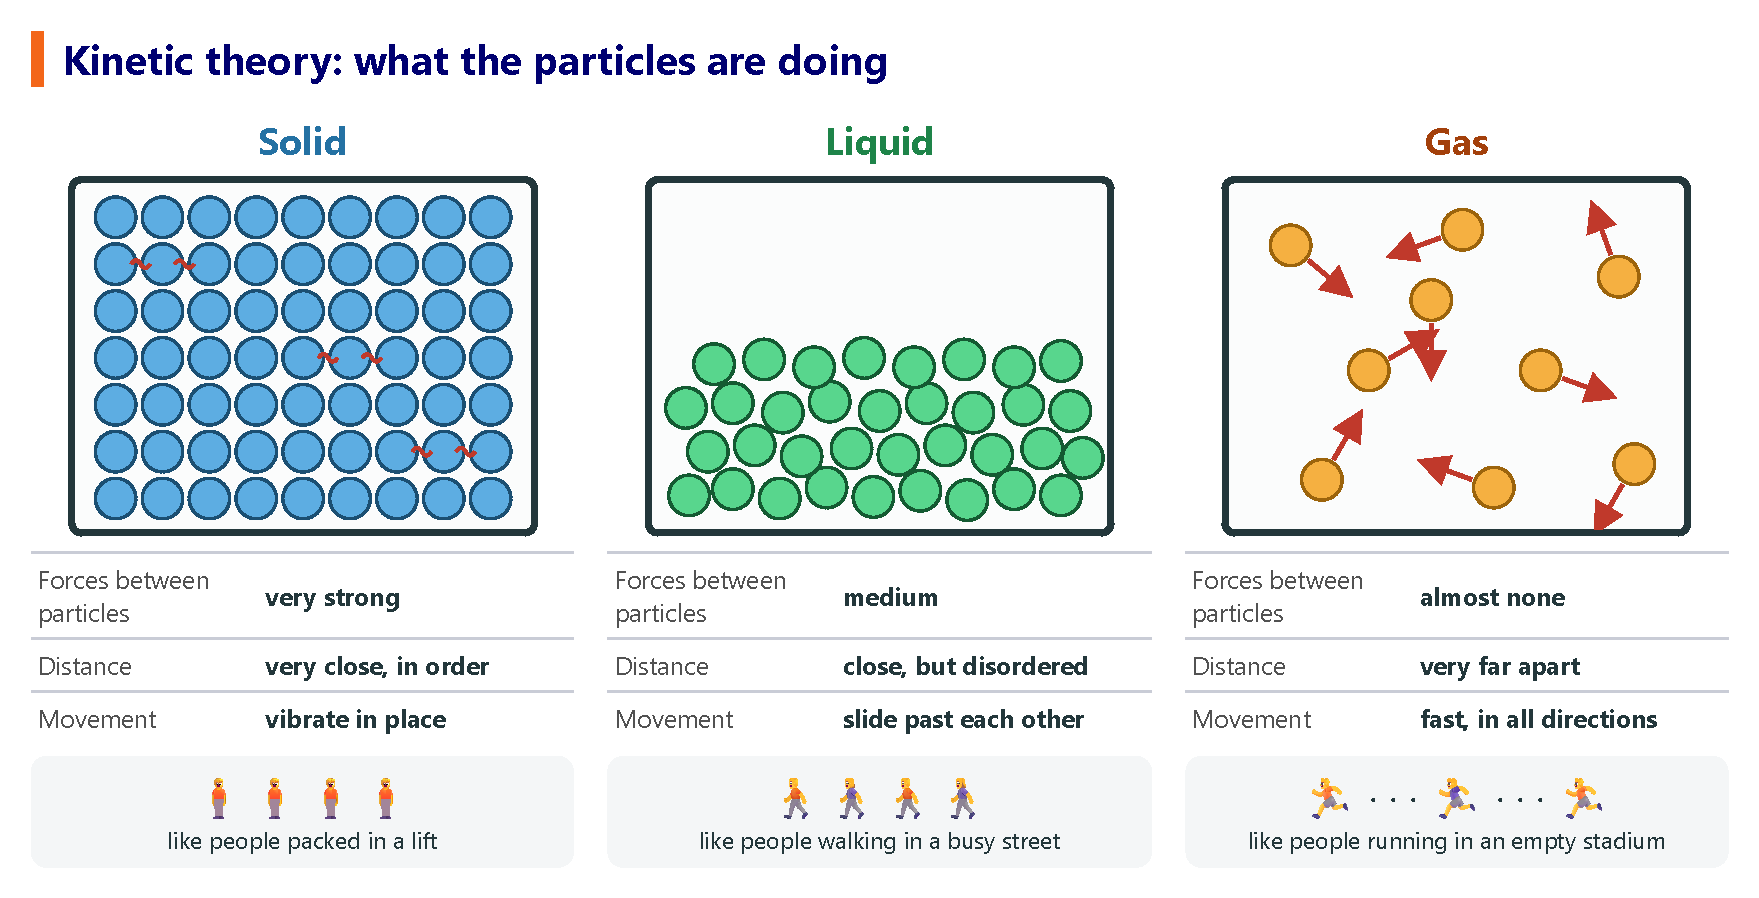
\includegraphics[width=\textwidth]{FigurasSVG/Unit_2_State_of_Matter/pdf/particle_model.pdf}
    \caption{The particle model of the three states of matter.}
    \label{fig:u2_particle_model}
\end{figure}

\begin{impt}
    Because their particles are so close together, solids usually have the \textbf{highest} density, liquids a little lower, and gases a \textbf{very low} density.
\end{impt}

\subsection{Gas pressure}

\begin{definition}[Pressure of a gas]
    The result of the particles of a gas \textbf{hitting the walls} of their container. More hits, or stronger hits, mean more pressure.
\end{definition}

\begin{figure}[H]
    \centering
    % [FIGURA ORIGINAL] \includegraphics[width=\textwidth]{Unit_2/gas_pressure}
    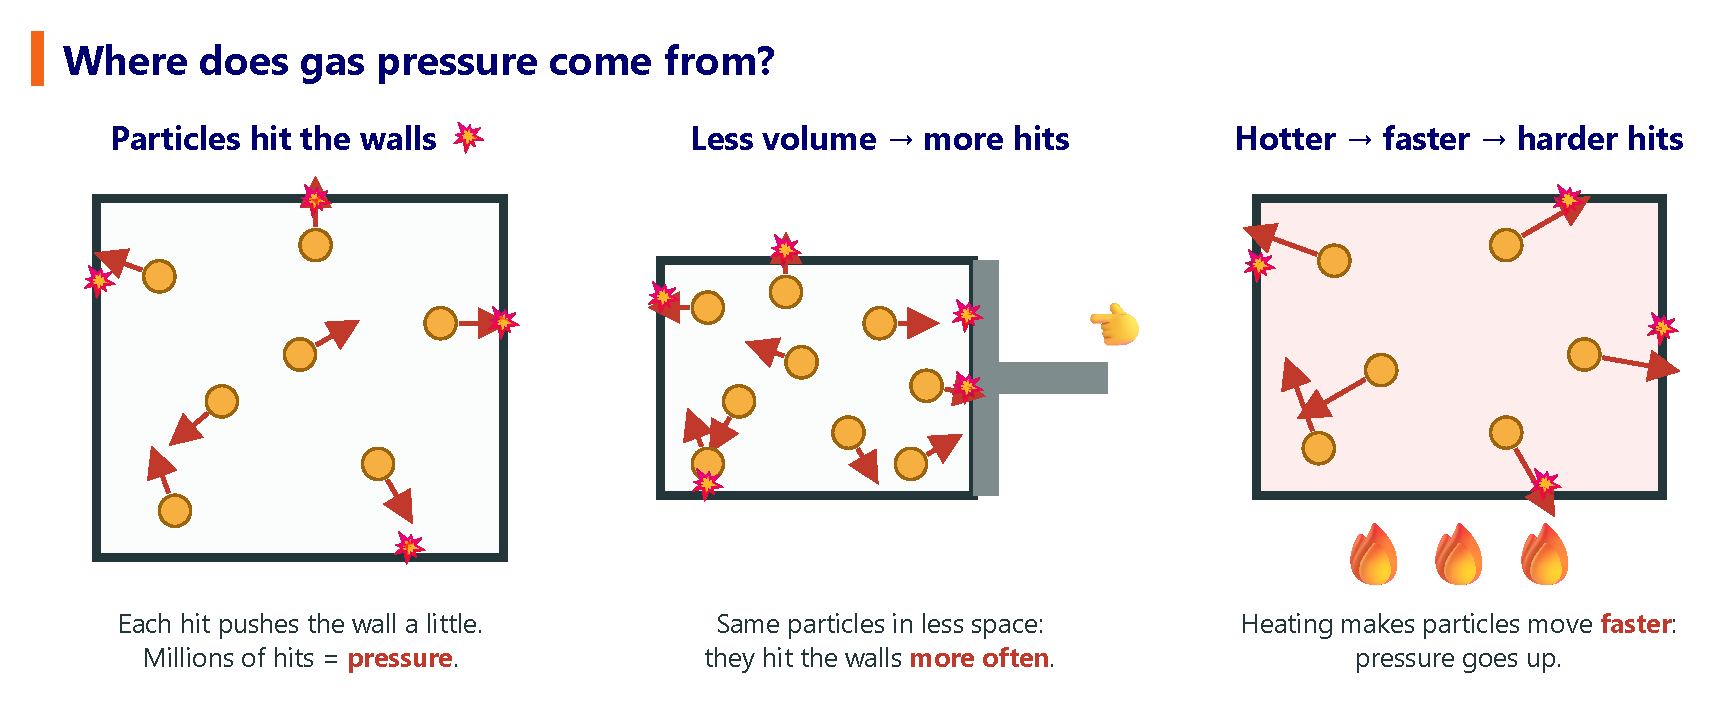
\includegraphics[width=\textwidth]{FigurasSVG/Unit_2_State_of_Matter/pdf/gas_pressure.pdf}
    \caption{Gas pressure increases if the volume decreases or the temperature increases.}
    \label{fig:u2_gas_pressure}
\end{figure}

\begin{exercise}
    Use kinetic theory to explain why a block of metal expands slightly when it is heated, but does not change its state of matter.
    \begin{solu}
        Heating makes the particles of the solid vibrate more, so the distance between them increases slightly; but the forces between the particles are still strong enough to keep the rigid structure, so the substance is still a solid, only a little larger.
    \end{solu}
\end{exercise}

\begin{exercise}
    An iceberg floats in the sea.
    \begin{enumerate}[label=\letraminuscula]
        \item Use kinetic theory to explain whether the particles are further apart in ice or in liquid water.
        \item What will happen to sea level if the iceberg melts?
    \end{enumerate}
    \begin{solu}
        \begin{enumerate}[label=\alph*)]
            \item Since ice floats, it is \textbf{less dense} than liquid water; therefore its particles are \textbf{further apart} in the solid than in the liquid (water is an unusual substance in this respect).
            \item The iceberg is already floating, so it already displaces a volume of water equal to its own weight; when it melts, sea level does \textbf{not} rise (unlike ice melting on land, which adds extra water to the sea).
        \end{enumerate}
    \end{solu}
\end{exercise}

\begin{exercise}
    The density of some gases at room temperature is: oxygen \qty{1.33}{\kg\per\cubic\metre}, helium \qty{0.17}{\kg\per\cubic\metre}, air \qty{1.20}{\kg\per\cubic\metre}. Explain why helium balloons float in air, while oxygen balloons would not.
    \begin{solu}
        A balloon floats in air when it is \textbf{less dense} than air. Helium (\qty{0.17}{\kg\per\cubic\metre}) is much less dense than air (\qty{1.20}{\kg\per\cubic\metre}), so it floats. Oxygen (\qty{1.33}{\kg\per\cubic\metre}) is denser than air, so an oxygen balloon would sink.
    \end{solu}
\end{exercise}

\begin{exercise}
    Two identical closed balloons are filled with the same amount of air. One is left in a fridge and the other next to a radiator. Use kinetic theory to predict which balloon will end up larger.
    \begin{solu}
        The balloon next to the \textbf{radiator}. Heat makes the air particles inside it move faster, so they hit the walls harder and more often; the pressure increases and pushes the walls outwards. In the cold balloon the particles move more slowly, the pressure is lower and the balloon stays smaller.
    \end{solu}
\end{exercise}

\subsection{Kinetic theory explains everyday phenomena}

\begin{figure}[H]
    \centering
    % [FIGURA ORIGINAL] \includegraphics[width=\textwidth]{Unit_2/everyday_kinetic}
    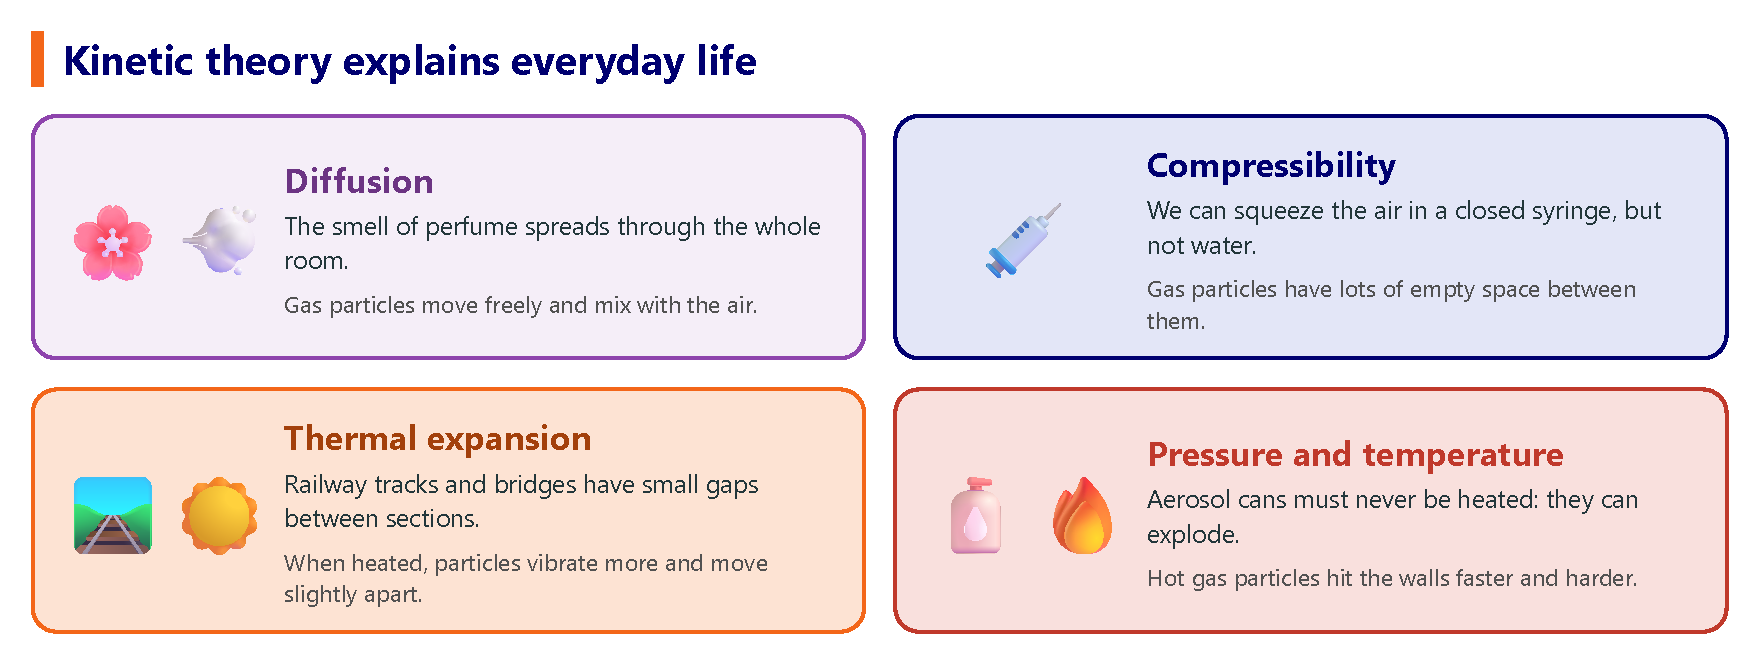
\includegraphics[width=\textwidth]{FigurasSVG/Unit_2_State_of_Matter/pdf/everyday_kinetic.pdf}
    \caption{Four everyday phenomena explained with particles.}
    \label{fig:u2_everyday_kinetic}
\end{figure}

\begin{definition}[Diffusion]
    The spreading of the particles of a substance until they mix completely with the particles of another one. It happens quickly in gases and more slowly in liquids (a drop of ink in water).
\end{definition}

\begin{exercise}
    Use kinetic theory (diffusion, expansion, compressibility) to explain each situation.
    \begin{enumerate}[label=\letraminuscula]
        \item You can smell food cooking in the kitchen from another room.
        \item A metal lid on a glass jar becomes easier to unscrew after running hot water over it.
        \item A bicycle pump becomes harder to push as you compress the air inside it.
    \end{enumerate}
    \begin{solu}
        \begin{enumerate}[label=\alph*)]
            \item The particles released by the food spread out by \textbf{diffusion} through the air until they reach your nose.
            \item Heat makes the metal particles in the lid vibrate more and move slightly apart, so the lid \textbf{expands} more than the glass and becomes looser.
            \item The same number of gas particles are squeezed into a smaller volume; they hit the piston more often, so the \textbf{pressure} (and the force needed to push) increases.
        \end{enumerate}
    \end{solu}
\end{exercise}

\begin{exercise}
    Perfume spreads across a room faster on a hot day than on a cold day. Use kinetic theory to explain why.
    \begin{solu}
        On a hot day the particles move \textbf{faster}, on average, than on a cold day. Diffusion is caused by the random motion of particles, so faster particles spread out and mix with the air more quickly.
    \end{solu}
\end{exercise}

\begin{exercise}
    A sealed bag of crisps looks normal at sea level, but when a plane climbs to cruising altitude, the same bag looks swollen.
    \begin{enumerate}[label=\letraminuscula]
        \item What happens to the air pressure outside the bag as the plane climbs?
        \item Use kinetic theory to explain why the bag swells up.
    \end{enumerate}
    \begin{solu}
        \begin{enumerate}[label=\alph*)]
            \item The air pressure \textbf{outside} the bag decreases as altitude increases.
            \item The air inside the bag keeps hitting the inner walls with the same force as before, while the air outside pushes back with less force. The outward push is greater, so the bag expands until the pressures balance (or it may even burst).
        \end{enumerate}
    \end{solu}
\end{exercise}

%----------------------------------------------------------------------------------------

\section{Gas laws}

The behaviour of a gas depends on three quantities: \textbf{pressure} \(p\), \textbf{volume} \(V\) and \textbf{temperature} \(T\). Each gas law keeps \textbf{one} of them constant and tells us how the other two are related.

\subsection{The Kelvin scale}

\begin{figure}[H]
    \centering
    % [FIGURA ORIGINAL] \includegraphics[width=0.95\textwidth]{Unit_2/kelvin_scale}
    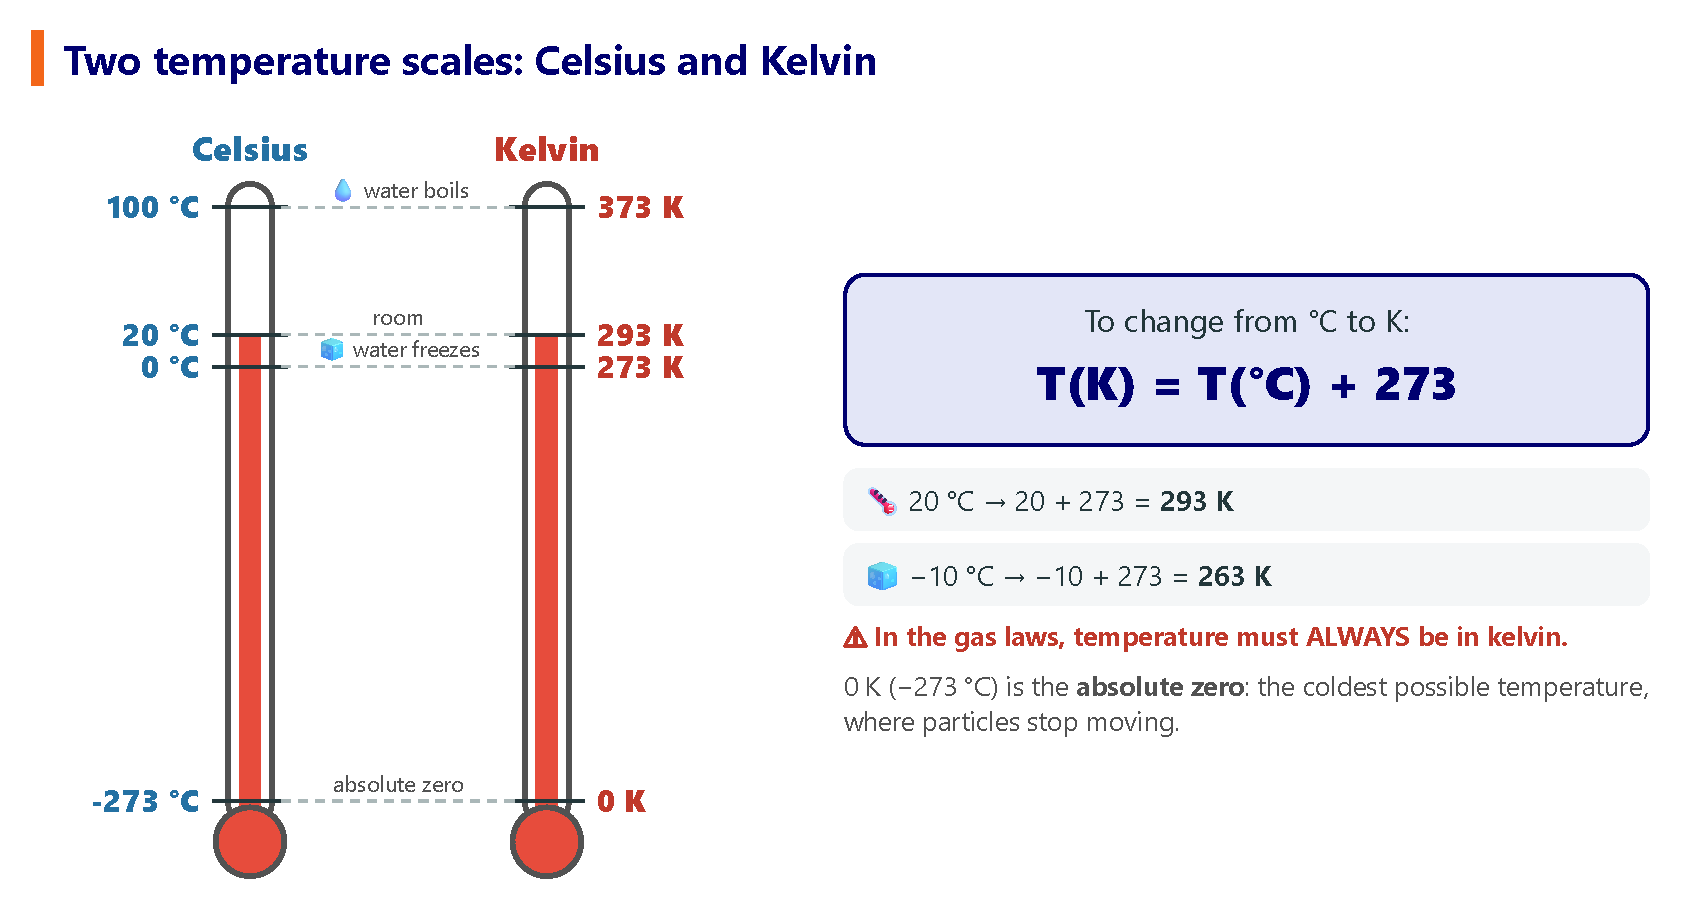
\includegraphics[width=0.95\textwidth]{FigurasSVG/Unit_2_State_of_Matter/pdf/kelvin_scale.pdf}
    \caption{The Celsius and Kelvin scales: same size of degree, different zero.}
    \label{fig:u2_kelvin_scale}
\end{figure}

\begin{impt}
    In \textbf{all} the gas laws, temperature must be in \textbf{kelvin}:
    \begin{equation*}
        T(\unit{\K}) = T(\unit{\celsius}) + 273
    \end{equation*}
\end{impt}

\subsection{What do the numbers 1 and 2 mean?}

In all the gas laws you will see the quantities written with a small number: \(p_1\), \(V_1\), \(T_1\) and \(p_2\), \(V_2\), \(T_2\). These small numbers are called \textbf{subscripts}, and they are very important:

\begin{impt}
    In the gas laws we always study the \textbf{same gas} at two different moments:
    \begin{itemize}
        \item The subscript \textbf{1} means the \textbf{beginning} (the \textbf{initial} state): how the gas is \textbf{before} the change.
        \item The subscript \textbf{2} means the \textbf{end} (the \textbf{final} state): how the gas is \textbf{after} something has changed (we heat it, cool it, compress it or let it expand).
    \end{itemize}
    For example, \(V_1\) is the volume \textbf{before} the change and \(V_2\) is the volume \textbf{after} the change.
\end{impt}

\begin{figure}[H]
    \centering
    % [FIGURA ORIGINAL] \includegraphics[width=\textwidth]{Unit_2/states_1_2}
    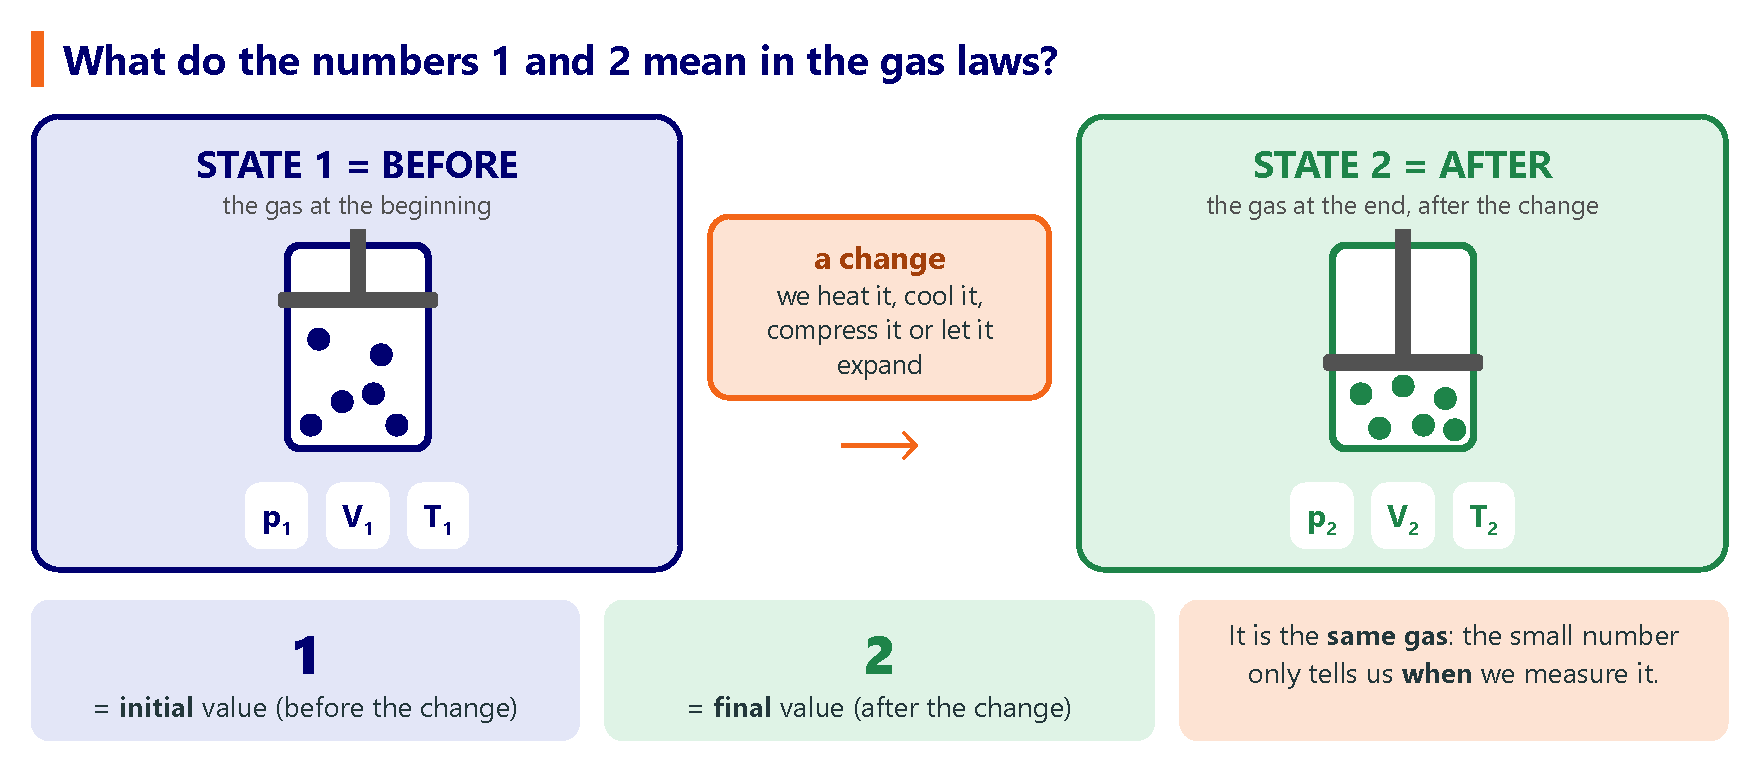
\includegraphics[width=\textwidth]{FigurasSVG/Unit_2_State_of_Matter/pdf/states_1_2.pdf}
    \caption{State 1 is the gas before the change; state 2 is the same gas after the change.}
    \label{fig:u2_states_1_2}
\end{figure}

\begin{example}
    \textbf{``A balloon has a volume of \qty{2}{\litre} at \qty{20}{\celsius}. We put it in the sun and it reaches \qty{40}{\celsius}.''} \\
    The \textbf{beginning} is the balloon before going into the sun: \(V_1 = \qty{2}{\litre}\), \(T_1 = \qty{20}{\celsius}\). \\
    The \textbf{end} is the balloon after being in the sun: \(T_2 = \qty{40}{\celsius}\), and \(V_2\) is what we would have to calculate.
\end{example}

\subsection{The three gas laws}

\begin{figure}[H]
    \centering
    % [FIGURA ORIGINAL] \includegraphics[width=\textwidth]{Unit_2/gas_laws}
    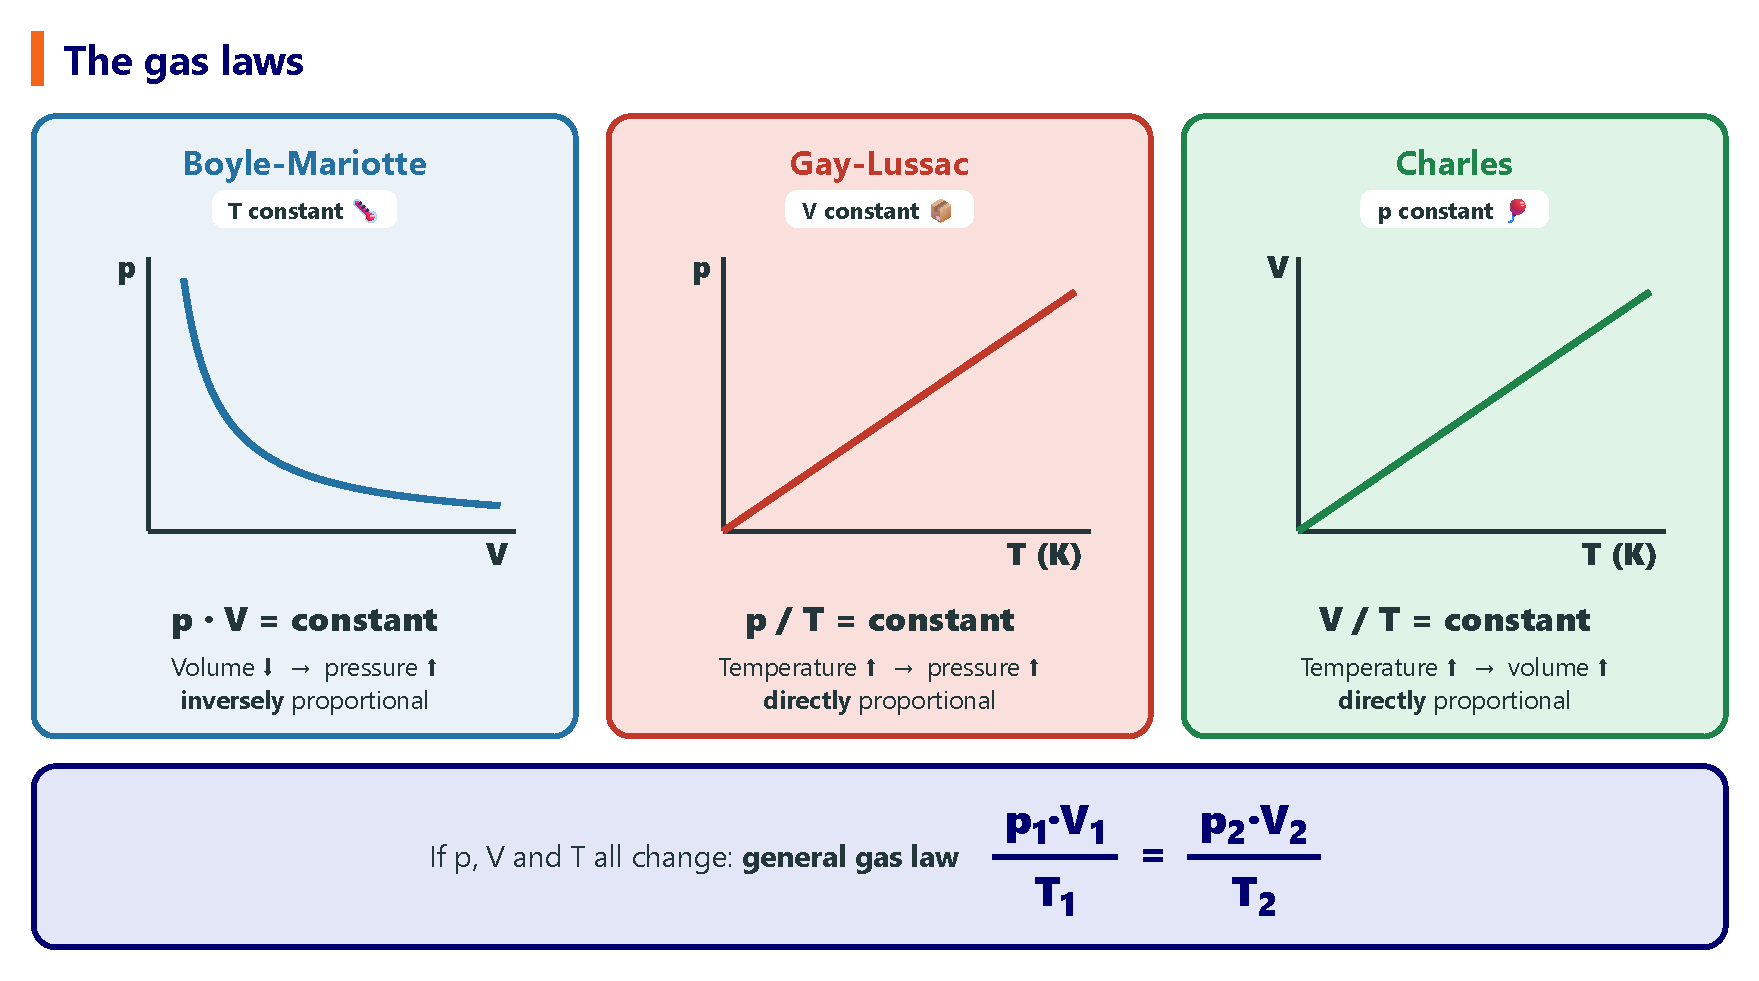
\includegraphics[width=\textwidth]{FigurasSVG/Unit_2_State_of_Matter/pdf/gas_laws.pdf}
    \caption{The three gas laws and the general gas law.}
    \label{fig:u2_gas_laws}
\end{figure}

\begin{table}[H]
    \centering
    \renewcommand{\arraystretch}{2}
    \begin{tabular}{lccc}
        \toprule
        \textbf{Law} & \textbf{Constant} & \textbf{Equation} & \textbf{Relationship} \\
        \midrule
        Boyle-Mariotte & \(T\) & \(p_1 \cdot V_1 = p_2 \cdot V_2\) & inversely proportional \\
        Gay-Lussac & \(V\) & \(\dfrac{p_1}{T_1} = \dfrac{p_2}{T_2}\) & directly proportional \\
        Charles & \(p\) & \(\dfrac{V_1}{T_1} = \dfrac{V_2}{T_2}\) & directly proportional \\
        \bottomrule
    \end{tabular}
    \caption{The gas laws.}
    \label{tab:u2_gas_laws}
\end{table}

\begin{impt}
    \negsubro{How do we know which law to use?} We look for the quantity that does \textbf{not} change (the one that stays \textbf{constant}):
    \begin{itemize}
        \item \(T\) constant \(\to\) \textbf{Boyle-Mariotte's law}.
        \item \(V\) constant \(\to\) \textbf{Gay-Lussac's law}.
        \item \(p\) constant \(\to\) \textbf{Charles' law}.
    \end{itemize}
    The complete method, step by step, is in the section \emph{Gas-law exercises}.
\end{impt}

%------------------------------------------------

\subsection{Boyle-Mariotte's law (constant temperature)}

\negsubro{What does this law tell us?} Take a bicycle pump, block the hole with your finger and push the handle. The more you push (the \textbf{smaller the volume}), the harder the air pushes back against your hand (the \textbf{bigger the pressure}).

Why does this happen? If the temperature of a gas does not change, its particles keep moving at the same speed. When we \textbf{compress} the gas, the particles have less space, so they hit the walls of the container \textbf{more often}: the \textbf{pressure increases}. If we let the gas \textbf{expand}, the particles have more space, they hit the walls less often and the pressure \textbf{decreases}.

We say that pressure and volume are \textbf{inversely proportional}: when one goes \textbf{up}, the other goes \textbf{down}. If the volume becomes half, the pressure becomes double; if the volume becomes double, the pressure becomes half.

\begin{definition}[Boyle-Mariotte's law]
    At constant temperature, the product of the pressure and the volume of a gas stays constant:
    \begin{equation*}
        p_1 \cdot V_1 = p_2 \cdot V_2
    \end{equation*}
\end{definition}

\begin{figure}[H]
    \centering
    % [FIGURA ORIGINAL] \includegraphics[width=\textwidth]{Unit_2/boyle_law}
    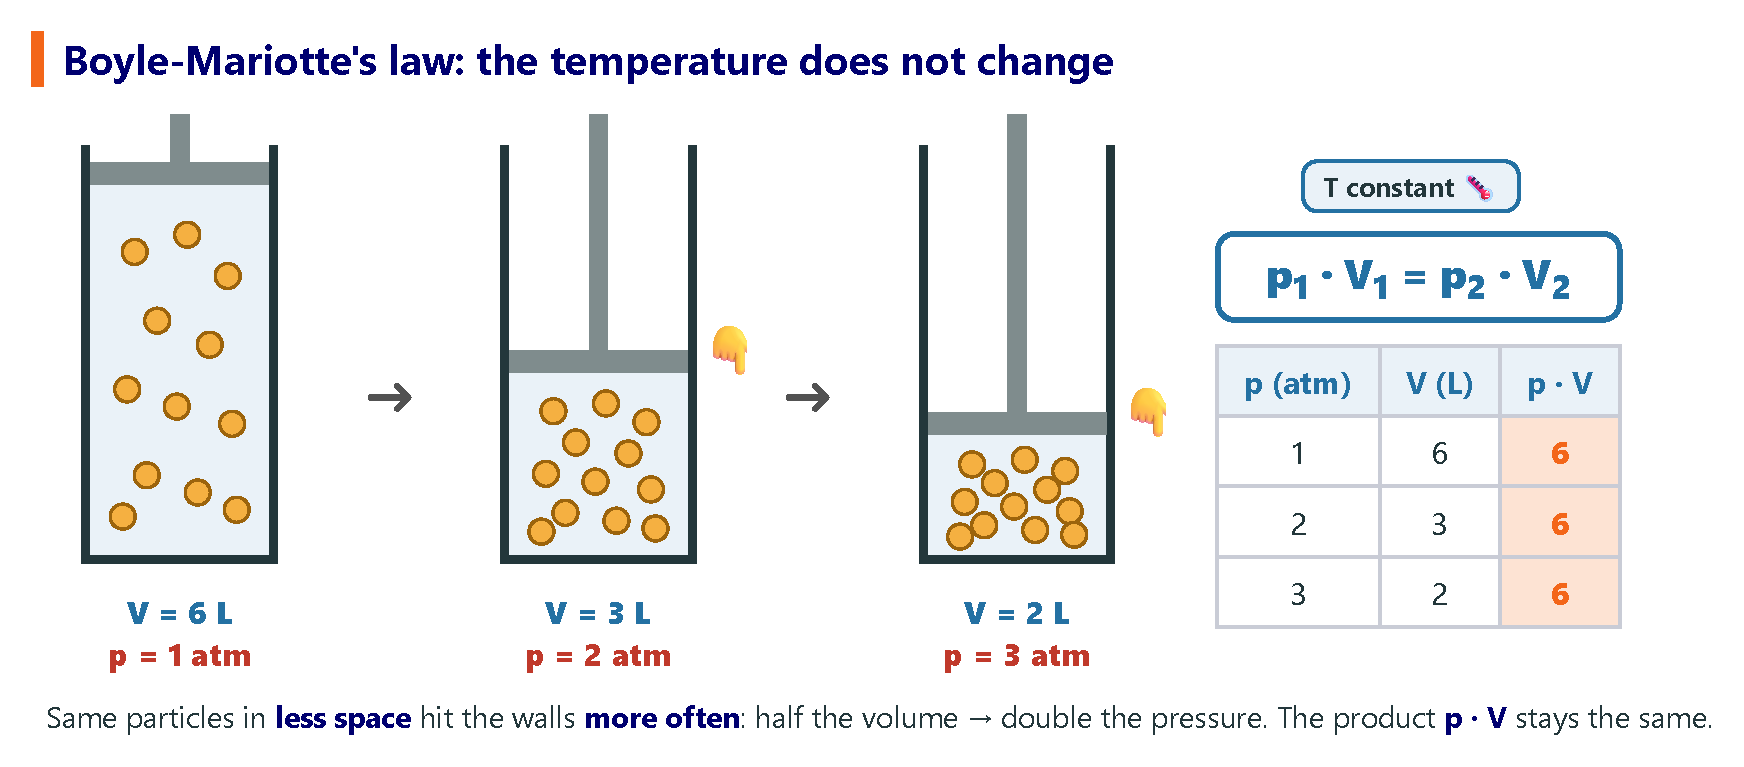
\includegraphics[width=\textwidth]{FigurasSVG/Unit_2_State_of_Matter/pdf/boyle_law.pdf}
    \caption{Boyle-Mariotte's law: at constant temperature, when the volume decreases the pressure increases, and \(p \cdot V\) stays the same.}
    \label{fig:u2_boyle_law}
\end{figure}

\begin{example}
    \textbf{In a \qty{3}{\litre} container, a gas exerts a pressure of \qty{2}{\atmospher} at \qty{60}{\celsius}. What will its volume be if the pressure doubles to \qty{4}{\atmospher} and the temperature stays the same?}
    \begin{enumerate}[label=\numberballmDarkTeal]
        \item Data: \(p_1 = \qty{2}{\atmospher}\), \(V_1 = \qty{3}{\litre}\), \(p_2 = \qty{4}{\atmospher}\). Unknown: \(\underline{V_2}\).
        \item \(T\) is constant \(\to\) \textbf{Boyle-Mariotte law}: \(p_1 \cdot V_1 = p_2 \cdot V_2\).
        \item We isolate \(V_2\) and calculate:
        \(\;V_2 = \dfrac{p_1 \cdot V_1}{p_2} = \dfrac{\qty{2}{\atmospher} \cdot \qty{3}{\litre}}{\qty{4}{\atmospher}} = \textcolor{red}{\qty{1.5}{\litre}}\)
    \end{enumerate}
    Pressure doubles, so volume halves: it makes sense!
\end{example}

\begin{exercise}
    In a \qty{3}{\litre} container, nitrogen exerts a pressure of \qty{4}{\atmospher}. What will the pressure be if the volume of the container doubles and the temperature stays the same?
    \begin{solu}
        \(T\) constant \(\to\) Boyle-Mariotte law: \(p_1 \cdot V_1 = p_2 \cdot V_2\). \\
        \(p_2 = \dfrac{p_1 \cdot V_1}{V_2} = \dfrac{\qty{4}{\atmospher} \cdot \qty{3}{\litre}}{\qty{6}{\litre}} = \qty{2}{\atmospher}\).
    \end{solu}
\end{exercise}

\begin{exercise}
    \qty{22.5}{\litre} of nitrogen at \qty{748}{\mmhg} are compressed until the pressure is \qty{725}{\mmhg}, at constant temperature. What is the new volume?
    \begin{solu}
        \(T\) constant \(\to\) Boyle-Mariotte law: \(p_1 \cdot V_1 = p_2 \cdot V_2\). \\
        \(V_2 = \dfrac{p_1 \cdot V_1}{p_2} = \dfrac{\qty{748}{\mmhg} \cdot \qty{22.5}{\litre}}{\qty{725}{\mmhg}} \approx \qty{23.2}{\litre}\).
    \end{solu}
\end{exercise}

\subsubsection{How to isolate each quantity in Boyle-Mariotte's law}

In an exercise the unknown can be any of the four quantities. We always start from the law, \(p_1 \cdot V_1 = p_2 \cdot V_2\), and leave the unknown \textbf{alone}. As we did with density, we do the \textbf{same operation on both sides}: if the unknown is \textbf{multiplied} by a quantity, we \textbf{divide} both sides by that quantity (or, with the shortcut, what is \textbf{multiplying} goes to the other side \textbf{dividing}).

\begin{figure}[H]
    \centering
    % [FIGURA ORIGINAL] \includegraphics[width=\textwidth]{Unit_2/boyle_isolate}
    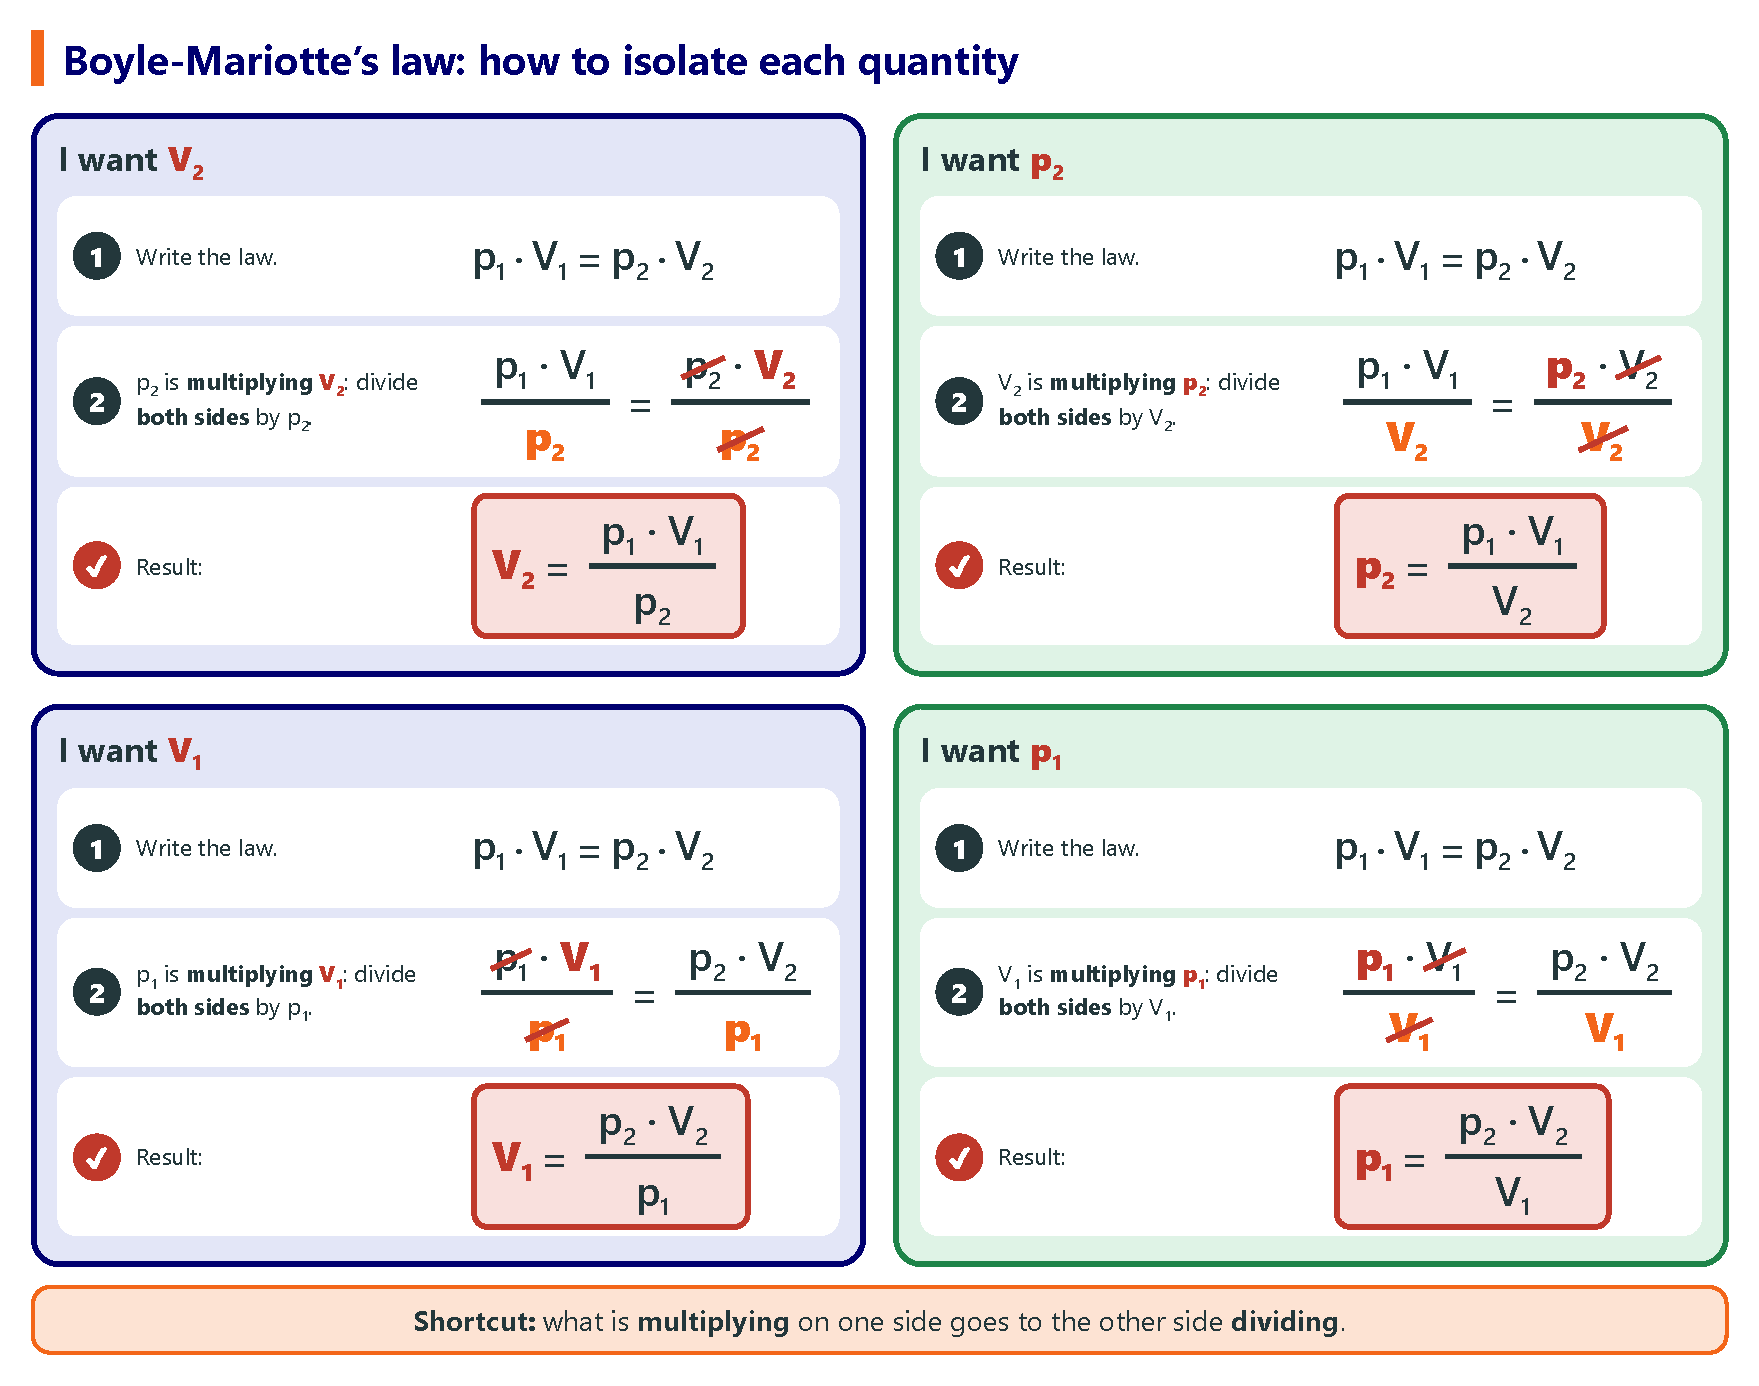
\includegraphics[width=\textwidth]{FigurasSVG/Unit_2_State_of_Matter/pdf/boyle_isolate.pdf}
    \caption{Isolating \(V_2\), \(p_2\), \(V_1\) and \(p_1\) in Boyle-Mariotte's law, step by step.}
    \label{fig:u2_boyle_isolate}
\end{figure}

\begin{itemize}
    \item \textbf{Unknown \(V_2\)}: \(p_2\) is multiplying \(V_2\), so we divide both sides by \(p_2\):
    \(\;\dfrac{p_1 \cdot V_1}{p_2} = \dfrac{\cancelred{p_2} \cdot V_2}{\cancelred{p_2}} \;\Rightarrow\; \textcolor{red}{V_2 = \dfrac{p_1 \cdot V_1}{p_2}}\)
    \item \textbf{Unknown \(p_2\)}: \(V_2\) is multiplying \(p_2\), so we divide both sides by \(V_2\):
    \(\;\dfrac{p_1 \cdot V_1}{V_2} = \dfrac{p_2 \cdot \cancelred{V_2}}{\cancelred{V_2}} \;\Rightarrow\; \textcolor{red}{p_2 = \dfrac{p_1 \cdot V_1}{V_2}}\)
    \item \textbf{Unknown \(V_1\)}: \(p_1\) is multiplying \(V_1\), so we divide both sides by \(p_1\):
    \(\;\dfrac{\cancelred{p_1} \cdot V_1}{\cancelred{p_1}} = \dfrac{p_2 \cdot V_2}{p_1} \;\Rightarrow\; \textcolor{red}{V_1 = \dfrac{p_2 \cdot V_2}{p_1}}\)
    \item \textbf{Unknown \(p_1\)}: \(V_1\) is multiplying \(p_1\), so we divide both sides by \(V_1\):
    \(\;\dfrac{p_1 \cdot \cancelred{V_1}}{\cancelred{V_1}} = \dfrac{p_2 \cdot V_2}{V_1} \;\Rightarrow\; \textcolor{red}{p_1 = \dfrac{p_2 \cdot V_2}{V_1}}\)
\end{itemize}

%------------------------------------------------

\subsection{Gay-Lussac's law (constant volume)}

\negsubro{What does this law tell us?} Have you noticed that spray cans have a warning: ``Do not leave in the sun or near a fire''? The can is made of metal, so the gas inside cannot change its volume. If it gets \textbf{hot}, the \textbf{pressure} of the gas \textbf{increases} so much that the can could explode.

Why does this happen? If a gas is inside a closed, rigid container, its volume cannot change. When we \textbf{heat} it, its particles move \textbf{faster} and hit the walls \textbf{harder and more often}: the \textbf{pressure increases}. When we cool it, the particles move more slowly and the pressure decreases.

We say that pressure and temperature (in kelvin) are \textbf{directly proportional}: when one goes \textbf{up}, the other goes \textbf{up} too. If the temperature in kelvin doubles, the pressure doubles too.

\begin{definition}[Gay-Lussac's law]
    At constant volume, the pressure of a gas divided by its temperature in kelvin stays constant:
    \begin{equation*}
        \dfrac{p_1}{T_1} = \dfrac{p_2}{T_2}
    \end{equation*}
\end{definition}

\begin{figure}[H]
    \centering
    % [FIGURA ORIGINAL] \includegraphics[width=\textwidth]{Unit_2/gay_lussac_law}
    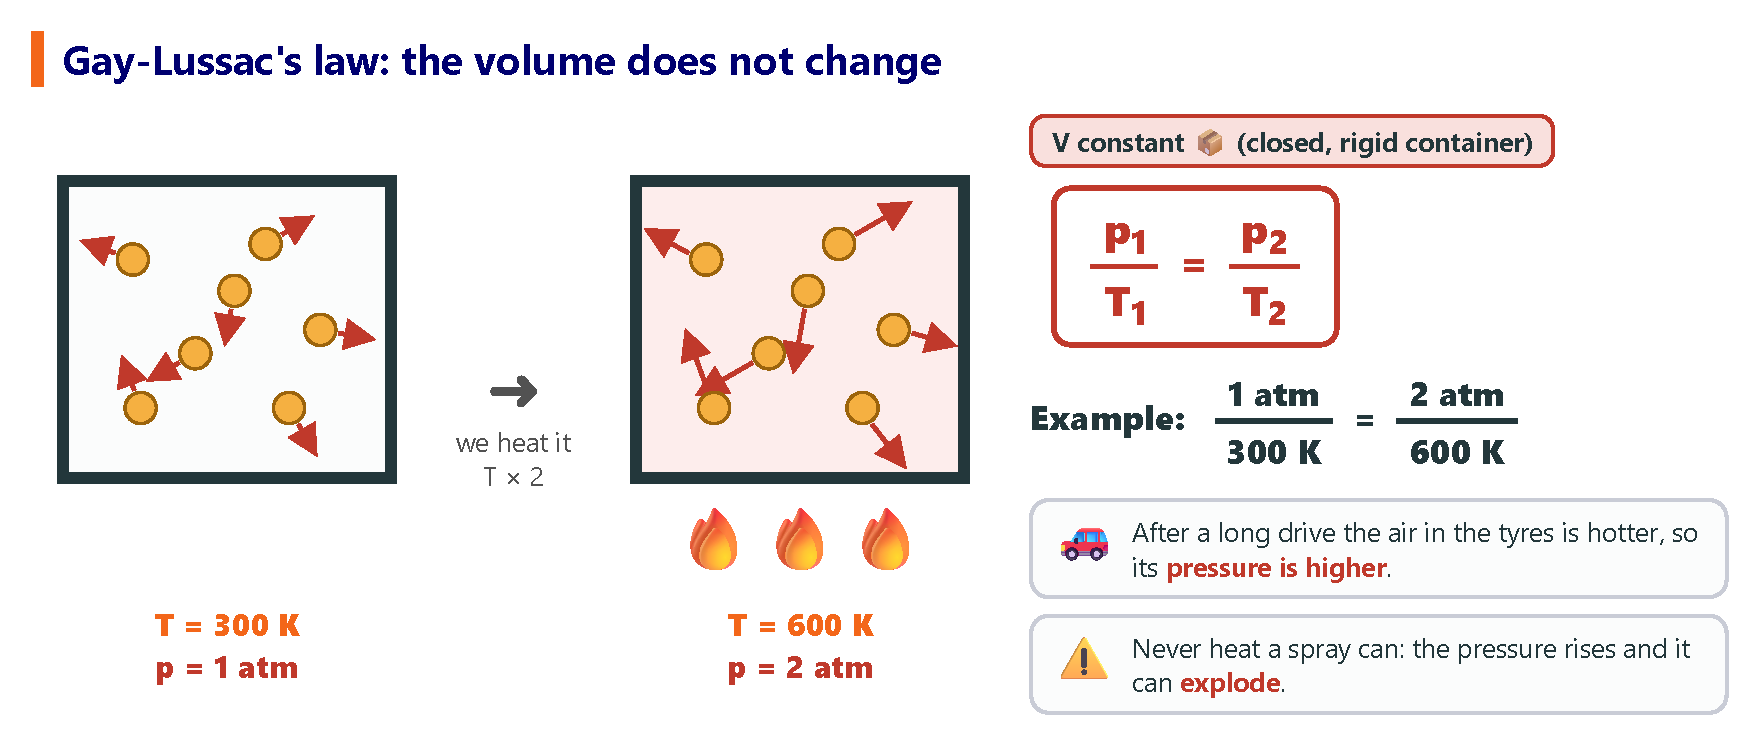
\includegraphics[width=\textwidth]{FigurasSVG/Unit_2_State_of_Matter/pdf/gay_lussac_law.pdf}
    \caption{Gay-Lussac's law: in a rigid container, if the temperature in kelvin doubles, the pressure doubles too.}
    \label{fig:u2_gay_lussac_law}
\end{figure}

\begin{example}
    \textbf{A closed container of gas is initially at \qty{0.500}{\atmospher} and \qty{25.0}{\celsius}. What will the pressure be at \qty{125.0}{\celsius}?}
    \begin{enumerate}[label=\numberballmDarkTeal]
        \item Data: \(p_1 = \qty{0.500}{\atmospher}\), \(T_1 = 25 + 273 = \qty{298}{\kelvin}\), \(T_2 = 125 + 273 = \qty{398}{\kelvin}\). Unknown: \(\underline{p_2}\).
        \item The container is closed, so \(V\) is constant \(\to\) \textbf{Gay-Lussac's law}: \(\dfrac{p_1}{T_1} = \dfrac{p_2}{T_2}\).
        \item We isolate \(p_2\) and calculate:
        \(\;p_2 = \dfrac{p_1 \cdot T_2}{T_1} = \dfrac{\qty{0.500}{\atmospher} \cdot \qty{398}{\kelvin}}{\qty{298}{\kelvin}} \approx \textcolor{red}{\qty{0.668}{\atmospher}}\)
    \end{enumerate}
    The temperature rises, so the pressure rises too: it makes sense!
\end{example}

\begin{exercise}
    In a \qty{10}{\litre} container, oxygen exerts a pressure of \qty{4}{\atmospher} at \qty{20}{\celsius}. What will the pressure be if the temperature rises to \qty{40}{\celsius} and the volume stays the same?
    \begin{solu}
        \(V\) constant \(\to\) Gay-Lussac's law: \(\dfrac{p_1}{T_1} = \dfrac{p_2}{T_2}\). \\
        In kelvin: \(T_1 = 20 + 273 = \qty{293}{\kelvin}\); \(T_2 = 40 + 273 = \qty{313}{\kelvin}\). \\
        \(p_2 = \dfrac{p_1 \cdot T_2}{T_1} = \dfrac{\qty{4}{\atmospher} \cdot \qty{313}{\kelvin}}{\qty{293}{\kelvin}} \approx \qty{4.27}{\atmospher}\).
    \end{solu}
\end{exercise}

\begin{exercise}
    A gas is cooled from \qty{323}{\kelvin} to \qty{273}{\kelvin} and its volume is kept constant. What is the final pressure if the original pressure was \qty{750.0}{\mmhg}?
    \begin{solu}
        \(V\) constant \(\to\) Gay-Lussac's law: \(\dfrac{p_1}{T_1} = \dfrac{p_2}{T_2}\). \\
        \(p_2 = \dfrac{p_1 \cdot T_2}{T_1} = \dfrac{\qty{750.0}{\mmhg} \cdot \qty{273}{\kelvin}}{\qty{323}{\kelvin}} \approx \qty{634}{\mmhg}\).
    \end{solu}
\end{exercise}

\subsubsection{How to isolate each quantity in Gay-Lussac's law}

We always start from the law, \(\dfrac{p_1}{T_1} = \dfrac{p_2}{T_2}\). Here the quantities are inside fractions, so we do it in two steps:
\begin{enumerate}[label=\numberballmDarkTeal]
    \item \textbf{We remove the fractions (cross-multiplication).} \(T_1\) is \textbf{dividing} on the left, so it goes to the right \textbf{multiplying}; \(T_2\) is \textbf{dividing} on the right, so it goes to the left \textbf{multiplying}:
    \begin{equation*}
        \dfrac{p_1}{T_1} = \dfrac{p_2}{T_2} \quad\Longrightarrow\quad p_1 \cdot T_2 = p_2 \cdot T_1
    \end{equation*}
    \item \textbf{We isolate the unknown}: the quantity that is \textbf{multiplying} the unknown goes to the other side \textbf{dividing} (we divide both sides by it).
\end{enumerate}

\begin{figure}[H]
    \centering
    % [FIGURA ORIGINAL] \includegraphics[width=\textwidth]{Unit_2/gay_lussac_isolate}
    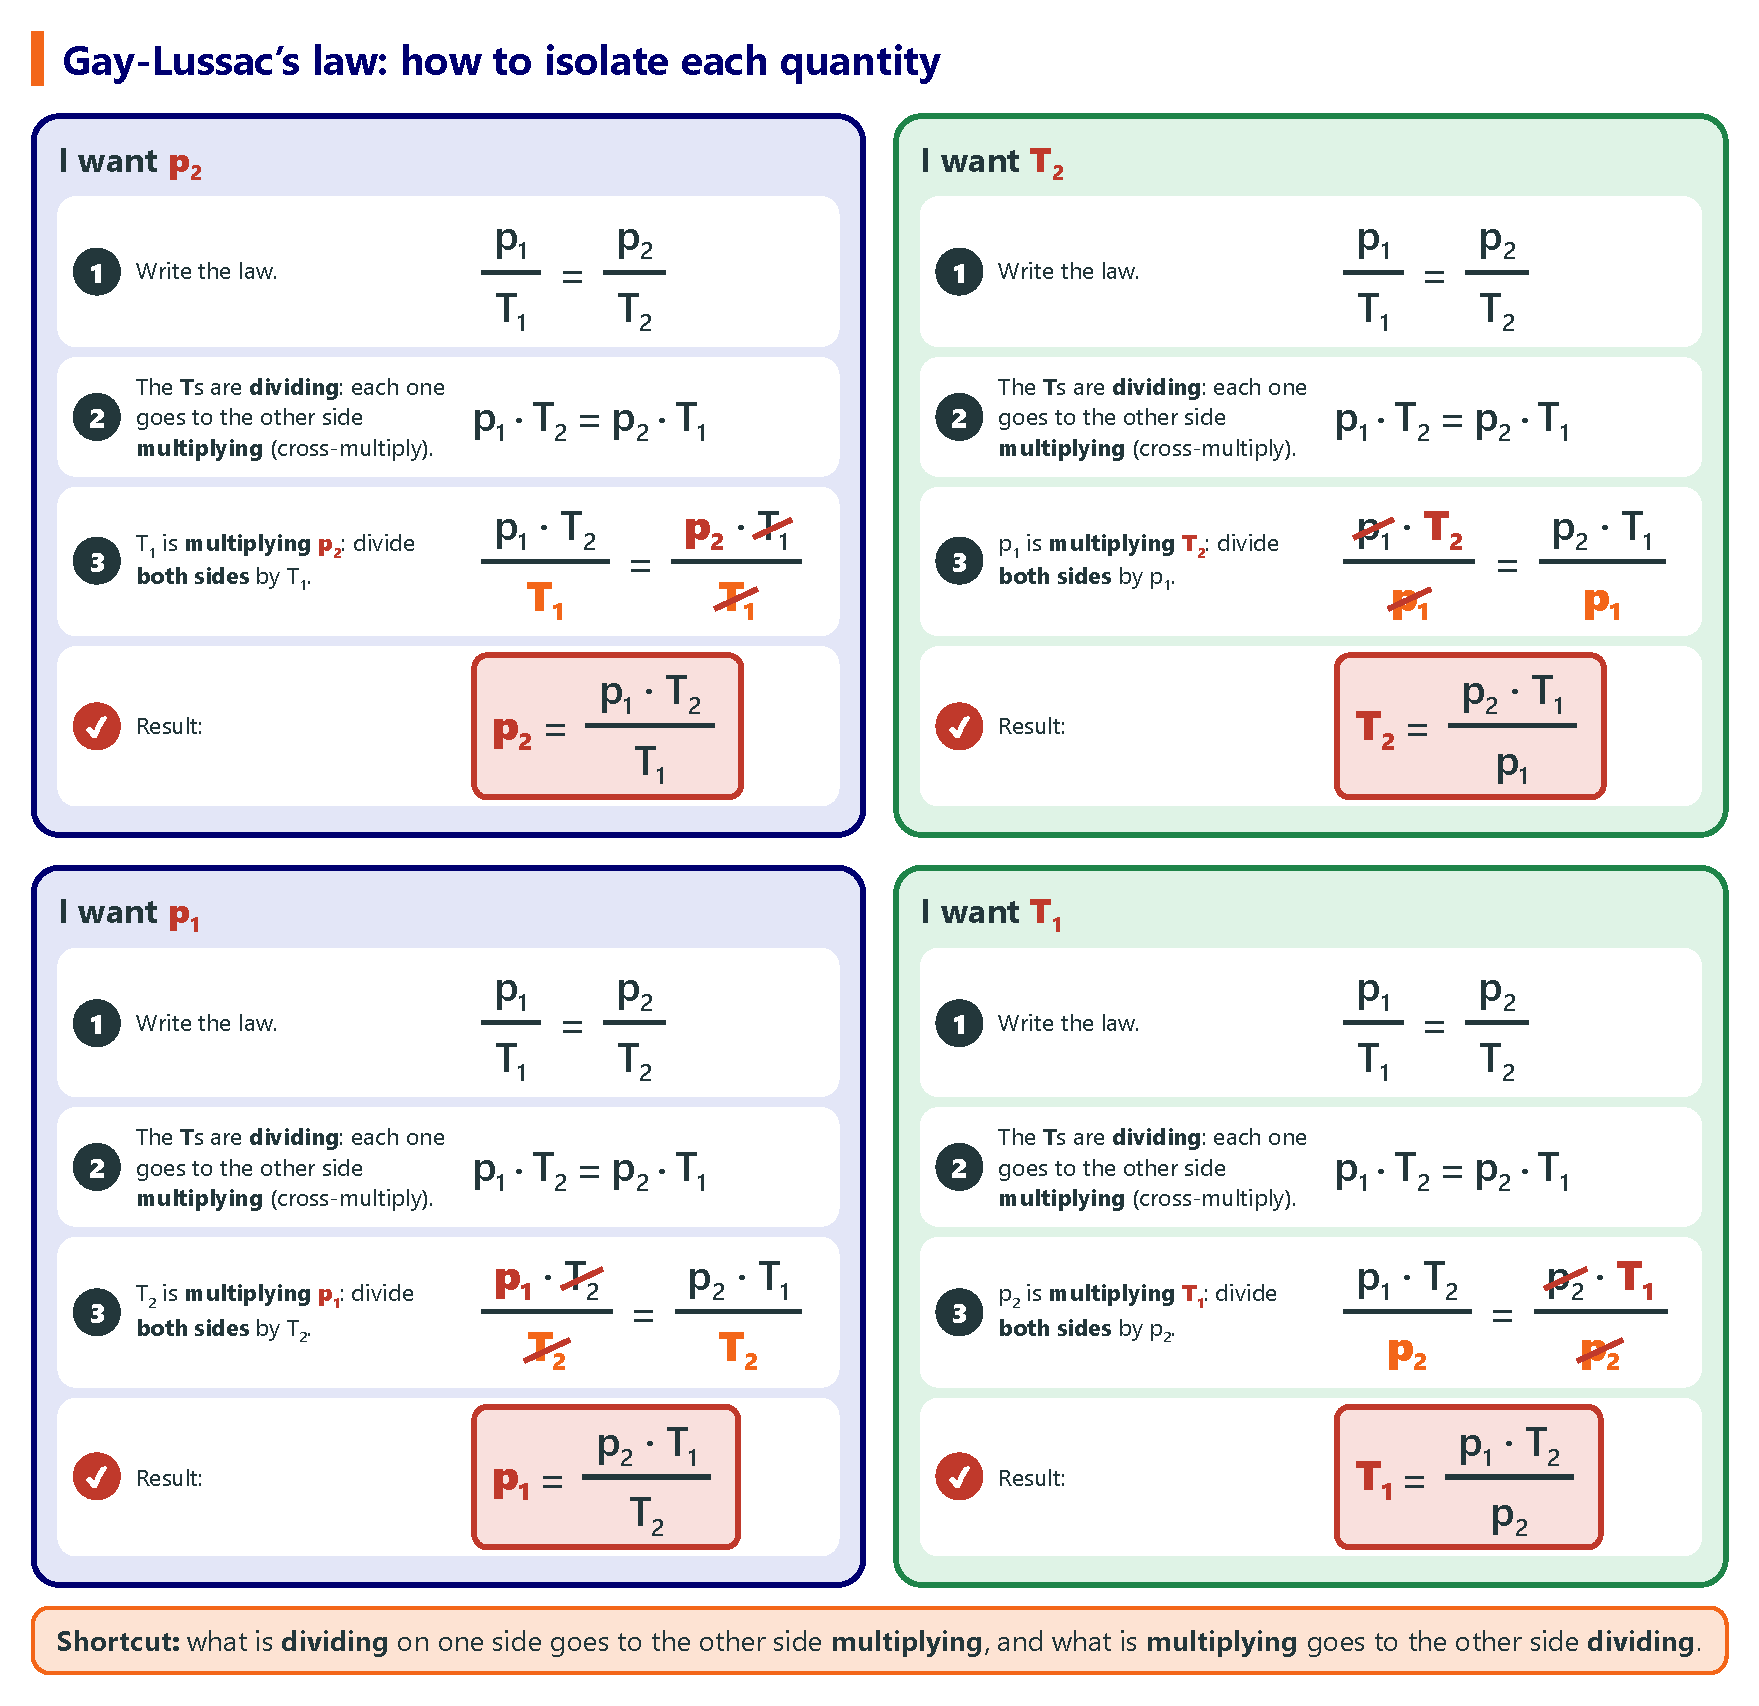
\includegraphics[width=\textwidth]{FigurasSVG/Unit_2_State_of_Matter/pdf/gay_lussac_isolate.pdf}
    \caption{Isolating the four quantities in Gay-Lussac's law, step by step.}
    \label{fig:u2_gay_lussac_isolate}
\end{figure}

Starting from \(p_1 \cdot T_2 = p_2 \cdot T_1\):
\begin{itemize}
    \item \textbf{Unknown \(p_2\)}: we divide both sides by \(T_1\):
    \(\;\dfrac{p_1 \cdot T_2}{T_1} = \dfrac{p_2 \cdot \cancelred{T_1}}{\cancelred{T_1}} \;\Rightarrow\; \textcolor{red}{p_2 = \dfrac{p_1 \cdot T_2}{T_1}}\)
    \item \textbf{Unknown \(T_2\)}: we divide both sides by \(p_1\):
    \(\;\dfrac{\cancelred{p_1} \cdot T_2}{\cancelred{p_1}} = \dfrac{p_2 \cdot T_1}{p_1} \;\Rightarrow\; \textcolor{red}{T_2 = \dfrac{p_2 \cdot T_1}{p_1}}\)
    \item \textbf{Unknown \(p_1\)}: we divide both sides by \(T_2\):
    \(\;\dfrac{p_1 \cdot \cancelred{T_2}}{\cancelred{T_2}} = \dfrac{p_2 \cdot T_1}{T_2} \;\Rightarrow\; \textcolor{red}{p_1 = \dfrac{p_2 \cdot T_1}{T_2}}\)
    \item \textbf{Unknown \(T_1\)}: we divide both sides by \(p_2\):
    \(\;\dfrac{p_1 \cdot T_2}{p_2} = \dfrac{\cancelred{p_2} \cdot T_1}{\cancelred{p_2}} \;\Rightarrow\; \textcolor{red}{T_1 = \dfrac{p_1 \cdot T_2}{p_2}}\)
\end{itemize}

%------------------------------------------------

\subsection{Charles' law (constant pressure)}

\negsubro{What does this law tell us?} Blow up a balloon and put it in the freezer: after a while it looks smaller and wrinkled. Take it out and leave it in the sun: it becomes big again. The \textbf{colder} the gas, the \textbf{smaller its volume}; the \textbf{hotter} the gas, the \textbf{bigger its volume}.

Why does this happen? Here the pressure of the gas does not change (a balloon or a syringe whose plunger can move freely). When we \textbf{heat} the gas, its particles move \textbf{faster} and push the walls \textbf{outwards}: the gas \textbf{expands} (its volume increases). When we cool it, the particles move more slowly and the gas \textbf{contracts}.

We say that volume and temperature (in kelvin) are \textbf{directly proportional}: when one goes \textbf{up}, the other goes \textbf{up} too. If the temperature in kelvin doubles, the volume doubles too.

\begin{definition}[Charles' law]
    At constant pressure, the volume of a gas divided by its temperature in kelvin stays constant:
    \begin{equation*}
        \dfrac{V_1}{T_1} = \dfrac{V_2}{T_2}
    \end{equation*}
\end{definition}

\begin{figure}[H]
    \centering
    % [FIGURA ORIGINAL] \includegraphics[width=\textwidth]{Unit_2/charles_law}
    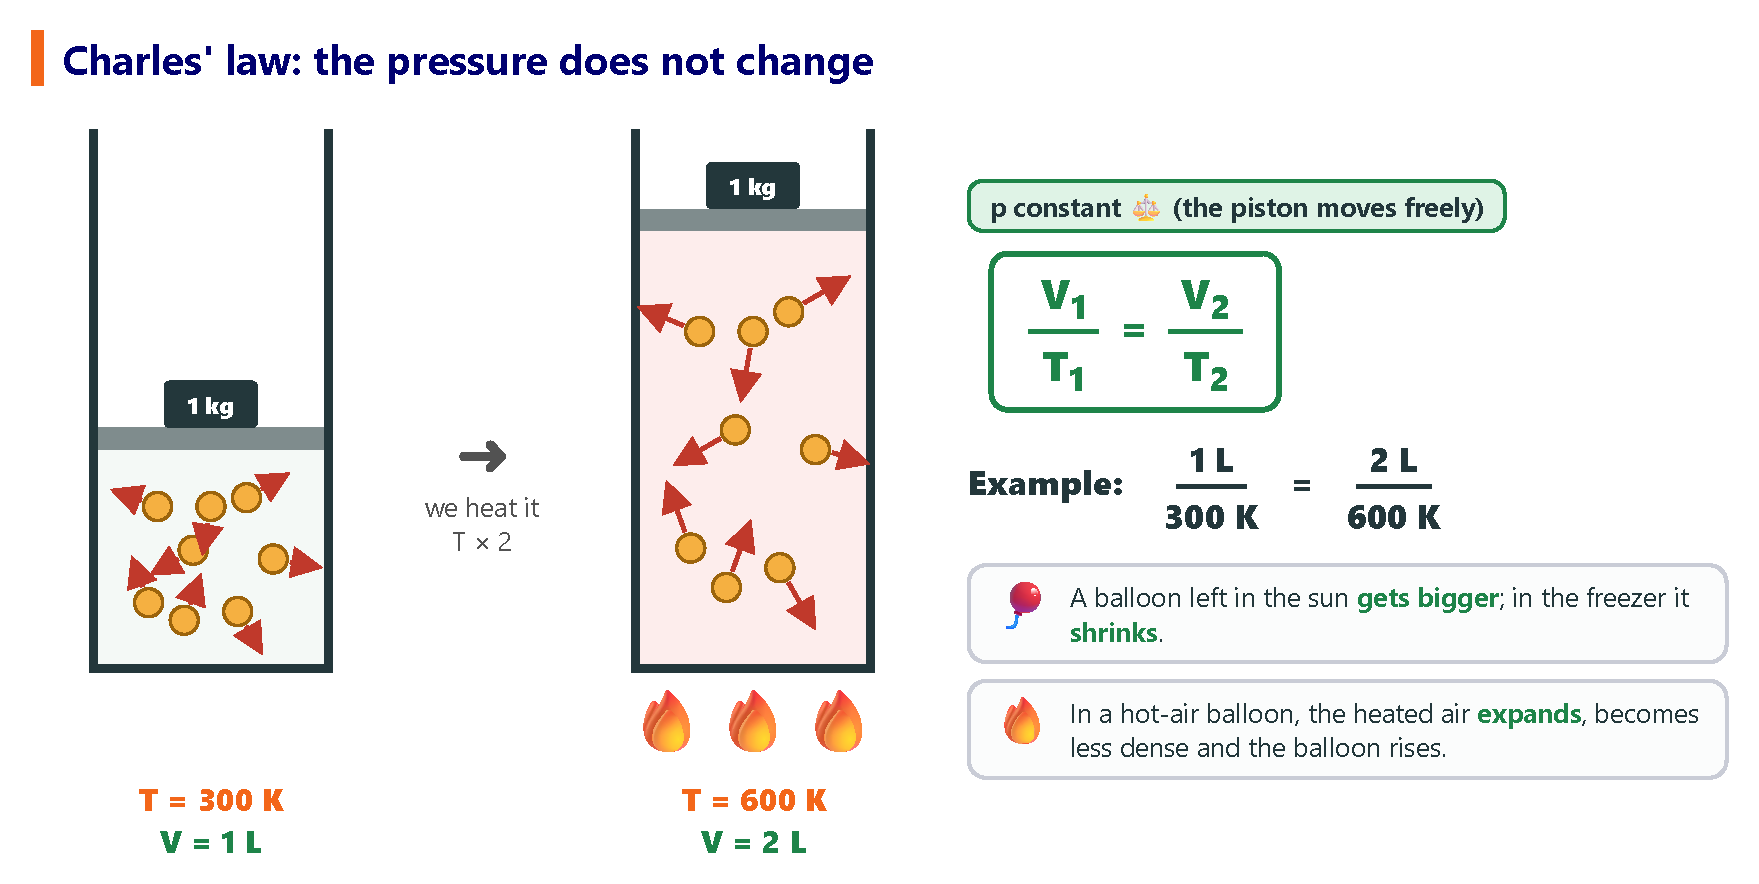
\includegraphics[width=\textwidth]{FigurasSVG/Unit_2_State_of_Matter/pdf/charles_law.pdf}
    \caption{Charles' law: with a free piston the pressure stays the same, and if the temperature in kelvin doubles, the volume doubles too.}
    \label{fig:u2_charles_law}
\end{figure}

\begin{example}
    \textbf{A gas occupies \qty{900.0}{\mL} at \qty{27.0}{\celsius}. What is its volume at \qty{132.0}{\celsius} if the pressure does not change?}
    \begin{enumerate}[label=\numberballmDarkTeal]
        \item Data: \(V_1 = \qty{900.0}{\mL}\), \(T_1 = 27 + 273 = \qty{300}{\kelvin}\), \(T_2 = 132 + 273 = \qty{405}{\kelvin}\). Unknown: \(\underline{V_2}\).
        \item \(p\) is constant \(\to\) \textbf{Charles' law}: \(\dfrac{V_1}{T_1} = \dfrac{V_2}{T_2}\).
        \item We isolate \(V_2\) and calculate:
        \(\;V_2 = \dfrac{V_1 \cdot T_2}{T_1} = \dfrac{\qty{900.0}{\mL} \cdot \qty{405}{\kelvin}}{\qty{300}{\kelvin}} = \textcolor{red}{\qty{1215}{\mL}}\)
    \end{enumerate}
    The temperature rises, so the gas expands: it makes sense!
\end{example}

\begin{exercise}
    A gas occupies \qty{2}{\litre} at \qty{300}{\kelvin}. What volume will it occupy if the temperature rises to \qty{450}{\kelvin}, with the pressure unchanged?
    \begin{solu}
        \(p\) constant \(\to\) Charles' law: \(\dfrac{V_1}{T_1} = \dfrac{V_2}{T_2}\). \\
        \(V_2 = \dfrac{V_1 \cdot T_2}{T_1} = \dfrac{\qty{2}{\litre} \cdot \qty{450}{\kelvin}}{\qty{300}{\kelvin}} = \qty{3}{\litre}\).
    \end{solu}
\end{exercise}

\begin{exercise}
    \qty{5.00}{\litre} of a gas are collected at \qty{100}{\kelvin} and then allowed to expand to \qty{20.0}{\litre}. What must the new temperature be to keep the same pressure?
    \begin{solu}
        \(p\) constant \(\to\) Charles' law: \(\dfrac{V_1}{T_1} = \dfrac{V_2}{T_2}\). \\
        \(T_2 = \dfrac{V_2 \cdot T_1}{V_1} = \dfrac{\qty{20.0}{\litre} \cdot \qty{100}{\kelvin}}{\qty{5.00}{\litre}} = \qty{400}{\kelvin}\).
    \end{solu}
\end{exercise}

\subsubsection{How to isolate each quantity in Charles' law}

We always start from the law, \(\dfrac{V_1}{T_1} = \dfrac{V_2}{T_2}\). Here the quantities are inside fractions, so we do it in two steps:
\begin{enumerate}[label=\numberballmDarkTeal]
    \item \textbf{We remove the fractions (cross-multiplication).} \(T_1\) is \textbf{dividing} on the left, so it goes to the right \textbf{multiplying}; \(T_2\) is \textbf{dividing} on the right, so it goes to the left \textbf{multiplying}:
    \begin{equation*}
        \dfrac{V_1}{T_1} = \dfrac{V_2}{T_2} \quad\Longrightarrow\quad V_1 \cdot T_2 = V_2 \cdot T_1
    \end{equation*}
    \item \textbf{We isolate the unknown}: the quantity that is \textbf{multiplying} the unknown goes to the other side \textbf{dividing} (we divide both sides by it).
\end{enumerate}

\begin{figure}[H]
    \centering
    % [FIGURA ORIGINAL] \includegraphics[width=\textwidth]{Unit_2/charles_isolate}
    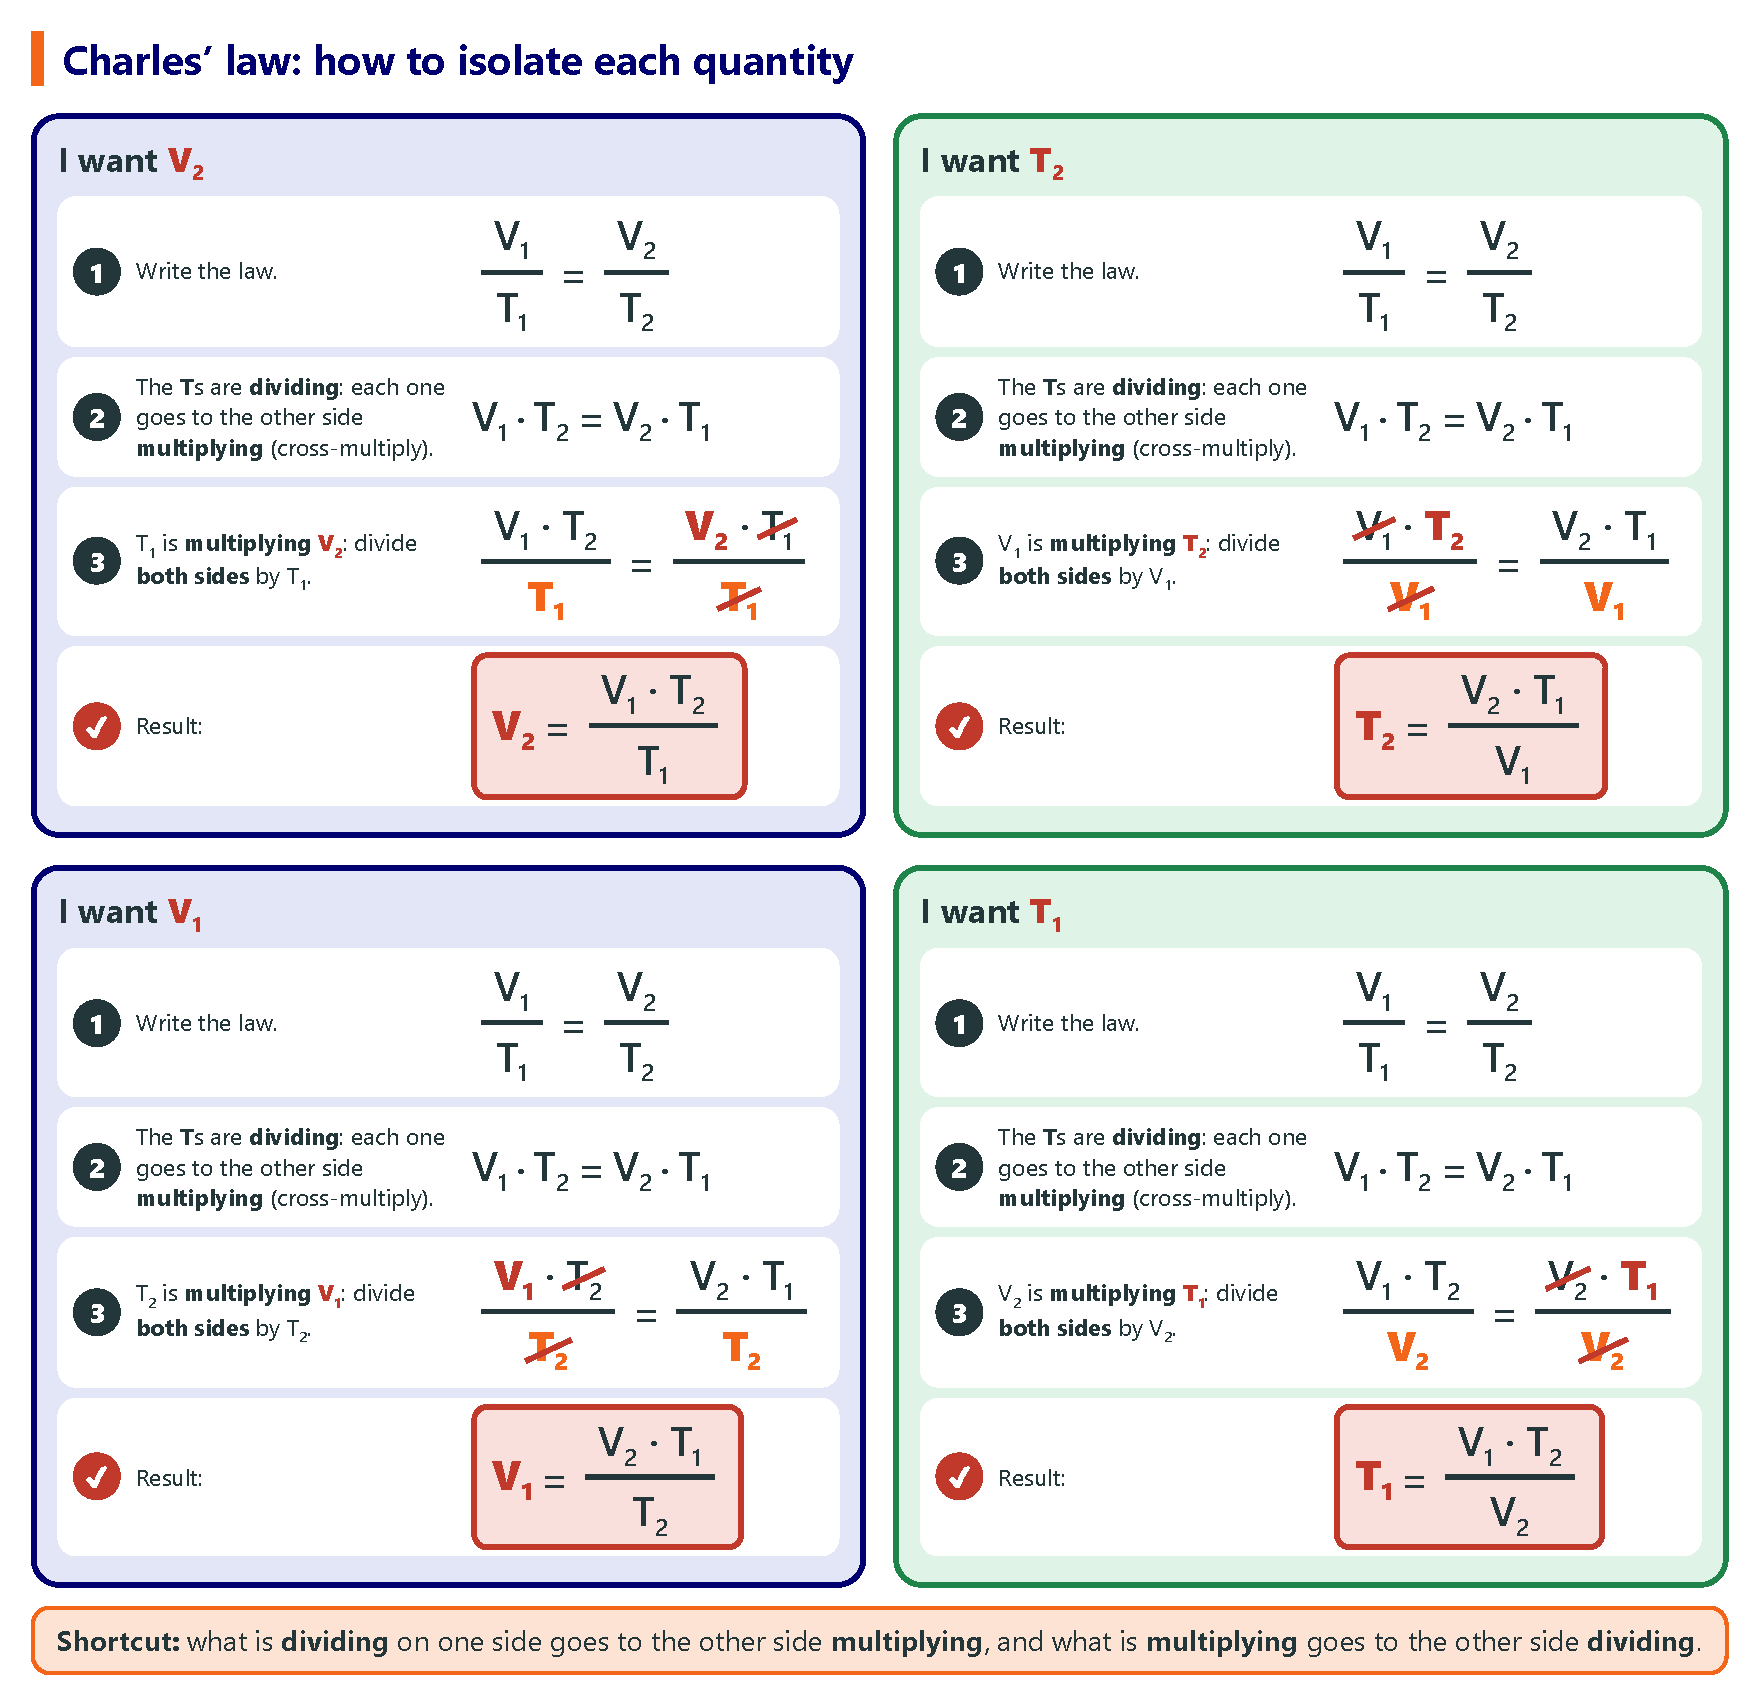
\includegraphics[width=\textwidth]{FigurasSVG/Unit_2_State_of_Matter/pdf/charles_isolate.pdf}
    \caption{Isolating the four quantities in Charles' law, step by step.}
    \label{fig:u2_charles_isolate}
\end{figure}

Starting from \(V_1 \cdot T_2 = V_2 \cdot T_1\):
\begin{itemize}
    \item \textbf{Unknown \(V_2\)}: we divide both sides by \(T_1\):
    \(\;\dfrac{V_1 \cdot T_2}{T_1} = \dfrac{V_2 \cdot \cancelred{T_1}}{\cancelred{T_1}} \;\Rightarrow\; \textcolor{red}{V_2 = \dfrac{V_1 \cdot T_2}{T_1}}\)
    \item \textbf{Unknown \(T_2\)}: we divide both sides by \(V_1\):
    \(\;\dfrac{\cancelred{V_1} \cdot T_2}{\cancelred{V_1}} = \dfrac{V_2 \cdot T_1}{V_1} \;\Rightarrow\; \textcolor{red}{T_2 = \dfrac{V_2 \cdot T_1}{V_1}}\)
    \item \textbf{Unknown \(V_1\)}: we divide both sides by \(T_2\):
    \(\;\dfrac{V_1 \cdot \cancelred{T_2}}{\cancelred{T_2}} = \dfrac{V_2 \cdot T_1}{T_2} \;\Rightarrow\; \textcolor{red}{V_1 = \dfrac{V_2 \cdot T_1}{T_2}}\)
    \item \textbf{Unknown \(T_1\)}: we divide both sides by \(V_2\):
    \(\;\dfrac{V_1 \cdot T_2}{V_2} = \dfrac{\cancelred{V_2} \cdot T_1}{\cancelred{V_2}} \;\Rightarrow\; \textcolor{red}{T_1 = \dfrac{V_1 \cdot T_2}{V_2}}\)
\end{itemize}

%------------------------------------------------

\subsection{Gas-law exercises}

In these exercises the laws are mixed. To solve them correctly, always follow the same procedure:

\negsubro{Method, step by step}:
\begin{enumerate}[label=\numberballmDarkTeal]
    \item \textbf{Read} the exercise \textbf{once}, to understand what is happening.
    \item \textbf{Read} the exercise \textbf{a second time}, looking for the numbers and their units.
    \item Draw a \textbf{table} with two columns: \textbf{Data} and \textbf{Unknown}.
    \item Write the \textbf{data} that the exercise gives you, saying whether each one belongs to the \textbf{beginning (1)} or to the \textbf{end (2)}: \(p_1\), \(V_1\), \(T_1\), \(p_2\)\ldots{} Change the temperatures to \textbf{kelvin}.
    \item In the \textbf{Unknown} column, write what the exercise asks for.
    \item Find the quantity that stays \textbf{constant}. It tells you which law you have to use: write its \textbf{name}.
    \item Write the \textbf{formula} of that law.
    \item \textbf{Isolate} the unknown in the formula.
    \item \textbf{Substitute} the numbers of each quantity (with their units), \textbf{calculate}, and check that the result makes sense.
\end{enumerate}

\begin{figure}[H]
    \centering
    % [FIGURA ORIGINAL] \includegraphics[width=\textwidth]{Unit_2/gas_law_method}
    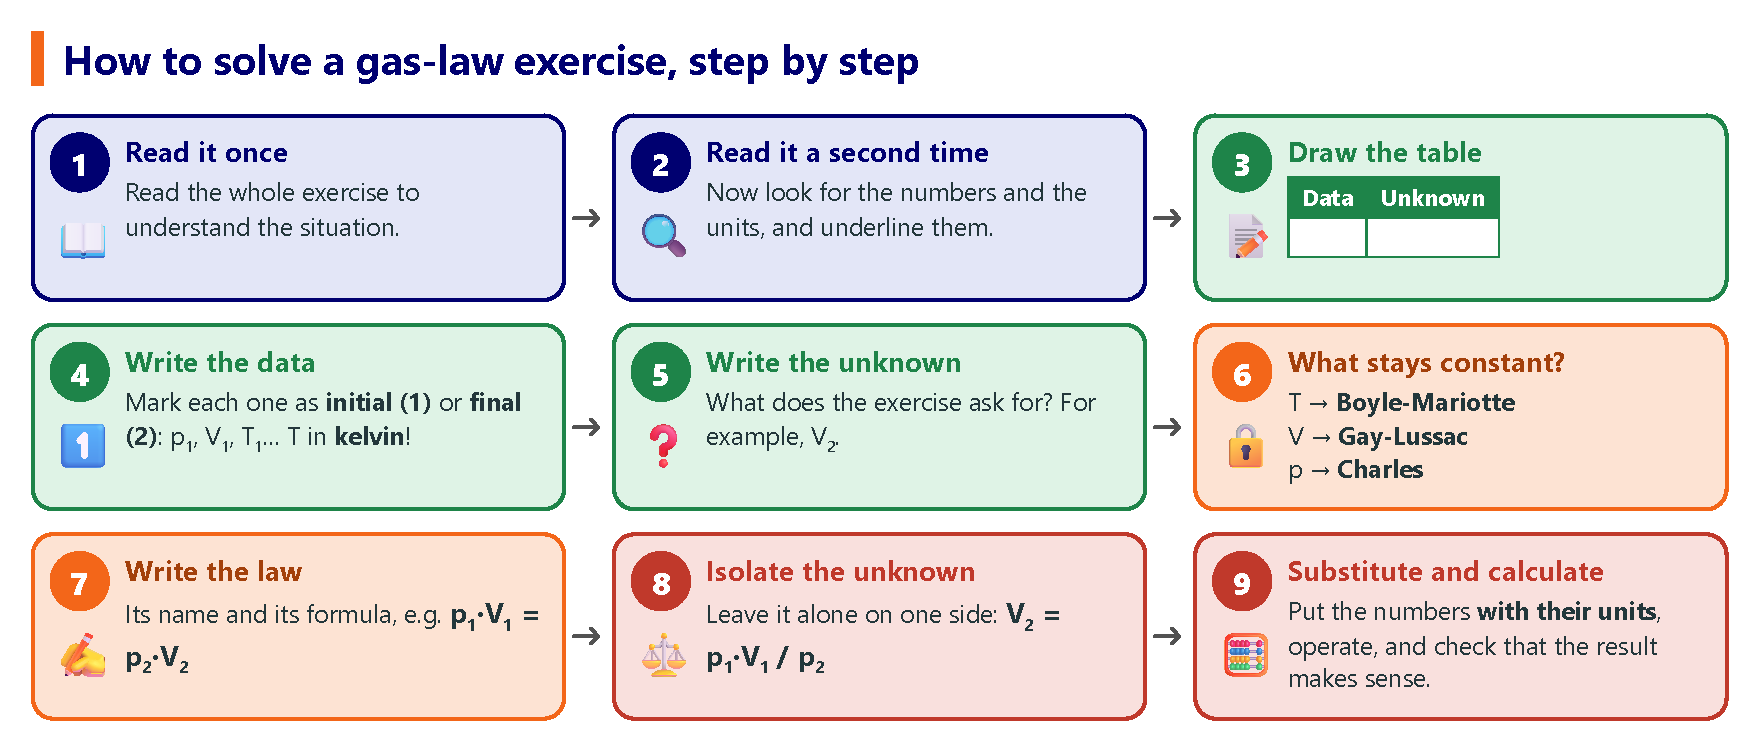
\includegraphics[width=\textwidth]{FigurasSVG/Unit_2_State_of_Matter/pdf/gas_law_method.pdf}
    \caption{The nine steps to solve a gas-law exercise.}
    \label{fig:u2_gas_law_method}
\end{figure}

\begin{example}
    \textbf{A gas occupies \qty{2.0}{\litre} at \qty{27}{\celsius}. It is heated to \qty{127}{\celsius} without changing its pressure. What is its final volume?}
    \begin{itemize}[leftmargin=2.3cm, labelwidth=2cm]
        \item[\textbf{Steps 1--2:}] We read the exercise twice: the gas is heated, and the pressure does not change.
        \item[\textbf{Steps 3--5:}] Table of data and unknown (temperatures in kelvin):
        \begin{center}
            \renewcommand{\arraystretch}{1.3}
            % --- tabla antigua ---
            % \begin{tabular}{l|l}
                % \textbf{Data} & \textbf{Unknown} \\
                % \hline
                % \(V_1 = \qty{2.0}{\litre}\) (beginning) & \(V_2 = \,?\) (end) \\
                % \(T_1 = 27 + 273 = \qty{300}{\kelvin}\) (beginning) & \\
                % \(T_2 = 127 + 273 = \qty{400}{\kelvin}\) (end) & \\
                % \(p\) = constant & \\
            % \end{tabular}
            % --- tabla nueva ---
            \begin{tabular}{@{}ll@{}}
                \toprule
                \textbf{Data} & \textbf{Unknown} \\
                \midrule
                \(V_1 = \qty{2.0}{\litre}\) (beginning) & \(V_2 = \,?\) (end) \\[3pt]
                \(T_1 = 27 + 273 = \qty{300}{\kelvin}\) (beginning) &  \\[3pt]
                \(T_2 = 127 + 273 = \qty{400}{\kelvin}\) (end) &  \\[3pt]
                \(p\) = constant &  \\
                \bottomrule
            \end{tabular}
        \end{center}
        \item[\textbf{Step 6:}] \(p\) is constant \(\to\) \textbf{Charles' law}.
        \item[\textbf{Step 7:}] Formula: \(\dfrac{V_1}{T_1} = \dfrac{V_2}{T_2}\).
        \item[\textbf{Step 8:}] We isolate \(V_2\): \(V_2 = \dfrac{V_1 \cdot T_2}{T_1}\).
        \item[\textbf{Step 9:}] \(V_2 = \dfrac{\qty{2.0}{\litre} \cdot \qty{400}{\kelvin}}{\qty{300}{\kelvin}} \approx \textcolor{red}{\qty{2.7}{\litre}}\). The gas is heated, so it expands: it makes sense!
    \end{itemize}
\end{example}

\begin{exercise}
    A gas with a volume of \qty{4}{\litre} at a pressure of \qty{205}{\kilo\pascal} is allowed to expand to a volume of \qty{12.0}{\litre}. What is the pressure in the container if the temperature remains constant?
    \begin{solu}
        \(T\) constant \(\to\) Boyle-Mariotte law. \\
        \(p_2 = \dfrac{p_1 \cdot V_1}{V_2} = \dfrac{\qty{205}{\kilo\pascal} \cdot \qty{4}{\litre}}{\qty{12.0}{\litre}} \approx \qty{68.3}{\kilo\pascal}\).
    \end{solu}
\end{exercise}

\begin{exercise}
    A closed, rigid gas container is initially at \qty{47}{\mmhg} and \qty{77}{\kelvin} (the temperature of liquid nitrogen). What will the pressure be when the container warms up to room temperature, \qty{25.0}{\celsius}?
    \begin{solu}
        \(V\) constant \(\to\) Gay-Lussac's law. \(T_2 = 25 + 273 = \qty{298}{\kelvin}\). \\
        \(p_2 = \dfrac{p_1 \cdot T_2}{T_1} = \dfrac{\qty{47}{\mmhg} \cdot \qty{298}{\kelvin}}{\qty{77}{\kelvin}} \approx \qty{182}{\mmhg}\).
    \end{solu}
\end{exercise}

\begin{exercise}
    \qty{15.0}{\litre} of neon at \qty{25.0}{\celsius} are allowed to expand to \qty{45.0}{\litre}. What must the new temperature be to keep the pressure constant?
    \begin{solu}
        \(p\) constant \(\to\) Charles' law. \(T_1 = 25 + 273 = \qty{298}{\kelvin}\). \\
        \(T_2 = \dfrac{V_2 \cdot T_1}{V_1} = \dfrac{\qty{45.0}{\litre} \cdot \qty{298}{\kelvin}}{\qty{15.0}{\litre}} = \qty{894}{\kelvin}\), that is, \(894 - 273 = \qty{621}{\celsius}\).
    \end{solu}
\end{exercise}

\begin{exercise}
    A gas at \qty{1.00}{\atmospher} is heated from \qty{20.0}{\celsius} to \qty{30.0}{\celsius} while its volume stays constant. Calculate the new pressure and how much the pressure has changed.
    \begin{solu}
        \(V\) constant \(\to\) Gay-Lussac's law. \(T_1 = 20 + 273 = \qty{293}{\kelvin}\); \(T_2 = 30 + 273 = \qty{303}{\kelvin}\). \\
        \(p_2 = \dfrac{p_1 \cdot T_2}{T_1} = \dfrac{\qty{1.00}{\atmospher} \cdot \qty{303}{\kelvin}}{\qty{293}{\kelvin}} \approx \qty{1.034}{\atmospher}\). \\
        The pressure increases by about \(\num{1.034} - \num{1.00} = \qty{0.034}{\atmospher}\).
    \end{solu}
\end{exercise}

\begin{exercise}
    A \qty{40}{\litre} tank of ammonia has a pressure of \qty{12.7}{\kilo\pascal}. Calculate the volume of the ammonia if its pressure changes to \qty{8.4}{\kilo\pascal} while its temperature remains constant.
    \begin{solu}
        \(T\) constant \(\to\) Boyle-Mariotte law. \\
        \(V_2 = \dfrac{p_1 \cdot V_1}{p_2} = \dfrac{\qty{12.7}{\kilo\pascal} \cdot \qty{40}{\litre}}{\qty{8.4}{\kilo\pascal}} \approx \qty{60.5}{\litre}\).
    \end{solu}
\end{exercise}

\begin{exercise}
    \qty{6.00}{\litre} of a gas at \qty{20.0}{\celsius} are compressed to \qty{4.00}{\litre} at constant pressure. Calculate the final temperature and how much the temperature has decreased.
    \begin{solu}
        \(p\) constant \(\to\) Charles' law. \(T_1 = 20 + 273 = \qty{293}{\kelvin}\). \\
        \(T_2 = \dfrac{V_2 \cdot T_1}{V_1} = \dfrac{\qty{4.00}{\litre} \cdot \qty{293}{\kelvin}}{\qty{6.00}{\litre}} \approx \qty{195}{\kelvin}\) (about \qty{-78}{\celsius}). \\
        The temperature decreases by about \(293 - 195 = \qty{98}{\kelvin}\), which is the same as \qty{98}{\celsius}, because a kelvin and a degree Celsius have the same size.
    \end{solu}
\end{exercise}

\begin{exercise}
    A gas thermometer measures temperature by measuring the pressure of a gas inside a container of fixed volume. The thermometer reads a pressure of \qty{248}{\kilo\pascal} at \qty{0}{\celsius}. What is the temperature when it reads a pressure of \qty{345}{\kilo\pascal}?
    \begin{solu}
        \(V\) constant \(\to\) Gay-Lussac's law. \(T_1 = 0 + 273 = \qty{273}{\kelvin}\). \\
        \(T_2 = \dfrac{p_2 \cdot T_1}{p_1} = \dfrac{\qty{345}{\kilo\pascal} \cdot \qty{273}{\kelvin}}{\qty{248}{\kilo\pascal}} \approx \qty{380}{\kelvin}\), that is, \(380 - 273 = \qty{107}{\celsius}\).
    \end{solu}
\end{exercise}

\begin{exercise}
    What pressure is needed to compress \qty{196.0}{\litre} of air at \qty{1.00}{\atmospher} into a cylinder whose volume is \qty{26}{\litre}, without changing its temperature?
    \begin{solu}
        \(T\) constant \(\to\) Boyle-Mariotte law. \\
        \(p_2 = \dfrac{p_1 \cdot V_1}{V_2} = \dfrac{\qty{1.00}{\atmospher} \cdot \qty{196.0}{\litre}}{\qty{26}{\litre}} \approx \qty{7.54}{\atmospher}\).
    \end{solu}
\end{exercise}

\begin{exercise}
    A gas is collected in a closed, rigid container at \qty{22.0}{\celsius} and \qty{745}{\mmhg}. When the temperature changes to \qty{0}{\celsius}, what is the new pressure?
    \begin{solu}
        \(V\) constant \(\to\) Gay-Lussac's law. \(T_1 = 22 + 273 = \qty{295}{\kelvin}\); \(T_2 = 0 + 273 = \qty{273}{\kelvin}\). \\
        \(p_2 = \dfrac{p_1 \cdot T_2}{T_1} = \dfrac{\qty{745}{\mmhg} \cdot \qty{273}{\kelvin}}{\qty{295}{\kelvin}} \approx \qty{689}{\mmhg}\).
    \end{solu}
\end{exercise}

\begin{exercise}
    A gas in a closed, rigid container has a pressure of \qty{699.0}{\mmhg} at \qty{40.0}{\celsius}. At what temperature will its pressure be \qty{1.00}{\atmospher}? (Remember: \(\qty{1}{\atmospher} = \qty{760}{\mmhg}\).)
    \begin{solu}
        \(V\) constant \(\to\) Gay-Lussac's law. \(T_1 = 40 + 273 = \qty{313}{\kelvin}\). \\
        Both pressures must be in the same unit: \(p_2 = \qty{1.00}{\atmospher} = \qty{760}{\mmhg}\). \\
        \(T_2 = \dfrac{p_2 \cdot T_1}{p_1} = \dfrac{\qty{760}{\mmhg} \cdot \qty{313}{\kelvin}}{\qty{699.0}{\mmhg}} \approx \qty{340}{\kelvin}\), that is, \(340 - 273 = \qty{67}{\celsius}\).
    \end{solu}
\end{exercise}

\begin{exercise}
    The temperature of a sample of gas in a steel tank at \qty{30}{\kilo\pascal} is increased from \qty{-100.0}{\celsius} to \qty{25.0}{\celsius}. What is the final pressure inside the tank?
    \begin{solu}
        A steel tank does not change its volume: \(V\) constant \(\to\) Gay-Lussac's law. \\
        \(T_1 = -100 + 273 = \qty{173}{\kelvin}\); \(T_2 = 25 + 273 = \qty{298}{\kelvin}\). \\
        \(p_2 = \dfrac{p_1 \cdot T_2}{T_1} = \dfrac{\qty{30}{\kilo\pascal} \cdot \qty{298}{\kelvin}}{\qty{173}{\kelvin}} \approx \qty{51.7}{\kilo\pascal}\).
    \end{solu}
\end{exercise}

%\subsection{General (combined) gas law}
%
%When \textbf{none} of the three quantities stays constant, we combine the three laws into one:
%
%\begin{equation*}
%    \dfrac{p_1 \cdot V_1}{T_1} = \dfrac{p_2 \cdot V_2}{T_2}
%\end{equation*}
%
%\begin{impt}
%    The three laws are special cases of this one: if \(T\) is constant it cancels and we get Boyle-Mariotte's law; if \(V\) is constant, Gay-Lussac's law; if \(p\) is constant, Charles' law. So you only need to remember \textbf{one} equation!
%\end{impt}
%
%\begin{example}
%    \textbf{A gas occupies \qty{2}{\litre} at \qty{1}{\atmospher} and \qty{27}{\celsius}. What volume will it occupy at \qty{2}{\atmospher} and \qty{127}{\celsius}?}
%
%    In kelvin: \(T_1 = 27 + 273 = \qty{300}{\kelvin}\); \(T_2 = 127 + 273 = \qty{400}{\kelvin}\).
%    \begin{equation*}
%        V_2 = \dfrac{p_1 \cdot V_1 \cdot T_2}{T_1 \cdot p_2} = \dfrac{\qty{1}{\atmospher} \cdot \qty{2}{\litre} \cdot \qty{400}{\kelvin}}{\qty{300}{\kelvin} \cdot \qty{2}{\atmospher}} = \textcolor{red}{\qty{1.33}{\litre}}
%    \end{equation*}
%\end{example}
%
%\begin{exercise}
%    A gas occupies \qty{4}{\litre} at \qty{2}{\atmospher} and \qty{300}{\kelvin}. What pressure will it exert if its volume is reduced to \qty{1}{\litre} and its temperature rises to \qty{600}{\kelvin}?
%    \begin{solu}
%        General gas law: \(p_2 = \dfrac{p_1 \cdot V_1 \cdot T_2}{T_1 \cdot V_2} = \dfrac{\qty{2}{\atmospher} \cdot \qty{4}{\litre} \cdot \qty{600}{\kelvin}}{\qty{300}{\kelvin} \cdot \qty{1}{\litre}} = \qty{16}{\atmospher}\).
%    \end{solu}
%\end{exercise}
%
%\begin{exercise}
%    A weather balloon is filled with helium at ground level, where \(p = \qty{1}{\atmospher}\), \(T = \qty{288}{\kelvin}\) (\qty{15}{\celsius}) and \(V = \qty{10}{\cubic\metre}\). It rises to a layer of the atmosphere where \(p = \qty{0.25}{\atmospher}\) and \(T = \qty{240}{\kelvin}\).
%    \begin{enumerate}[label=\letraminuscula]
%        \item Which gas law must be used, and why?
%        \item Calculate the new volume.
%    \end{enumerate}
%    \begin{solu}
%        \begin{enumerate}[label=\alph*)]
%            \item \(p\), \(V\) \textbf{and} \(T\) all change, so we must use the \textbf{general gas law}.
%            \item \(V_2 = \dfrac{p_1 \cdot V_1 \cdot T_2}{T_1 \cdot p_2} = \dfrac{\qty{1}{\atmospher} \cdot \qty{10}{\cubic\metre} \cdot \qty{240}{\kelvin}}{\qty{288}{\kelvin} \cdot \qty{0.25}{\atmospher}} \approx \qty{33.3}{\cubic\metre}\). The balloon expands a lot as it rises; that is why weather balloons eventually burst.
%        \end{enumerate}
%    \end{solu}
%\end{exercise}
%
%\begin{exercise}
%    A gas occupies \qty{5}{\litre} at \qty{2}{\atmospher} and \qty{250}{\kelvin}. What volume will it occupy at \qty{1}{\atmospher} and \qty{500}{\kelvin}?
%    \begin{solu}
%        \(V_2 = \dfrac{p_1 \cdot V_1 \cdot T_2}{T_1 \cdot p_2} = \dfrac{\qty{2}{\atmospher} \cdot \qty{5}{\litre} \cdot \qty{500}{\kelvin}}{\qty{250}{\kelvin} \cdot \qty{1}{\atmospher}} = \qty{20}{\litre}\).
%    \end{solu}
%\end{exercise}
%
%\begin{exercise}
%    In the morning, the air inside a car tyre is at \qty{280}{\kelvin}, occupies \qty{12}{\litre} and has a pressure of \qty{2}{\atmospher}. After driving for an hour, the air is at \qty{308}{\kelvin} and the tyre has expanded slightly to \qty{12.3}{\litre}.
%    \begin{enumerate}[label=\letraminuscula]
%        \item Which gas law should be applied here?
%        \item Calculate the new pressure of the air inside the tyre.
%    \end{enumerate}
%    \begin{solu}
%        \begin{enumerate}[label=\alph*)]
%            \item \(p\), \(V\) and \(T\) all change: the \textbf{general gas law}.
%            \item \(p_2 = \dfrac{p_1 \cdot V_1 \cdot T_2}{T_1 \cdot V_2} = \dfrac{\qty{2}{\atmospher} \cdot \qty{12}{\litre} \cdot \qty{308}{\kelvin}}{\qty{280}{\kelvin} \cdot \qty{12.3}{\litre}} \approx \qty{2.15}{\atmospher}\). This is why tyre pressure should be checked when the tyres are cold.
%        \end{enumerate}
%    \end{solu}
%\end{exercise}

%----------------------------------------------------------------------------------------

\section{Changes of state}

If we heat or cool a substance enough, it changes state. Each change has its own name:

\begin{figure}[H]
    \centering
    % [FIGURA ORIGINAL] \includegraphics[width=0.95\textwidth]{Unit_2/changes_of_state}
    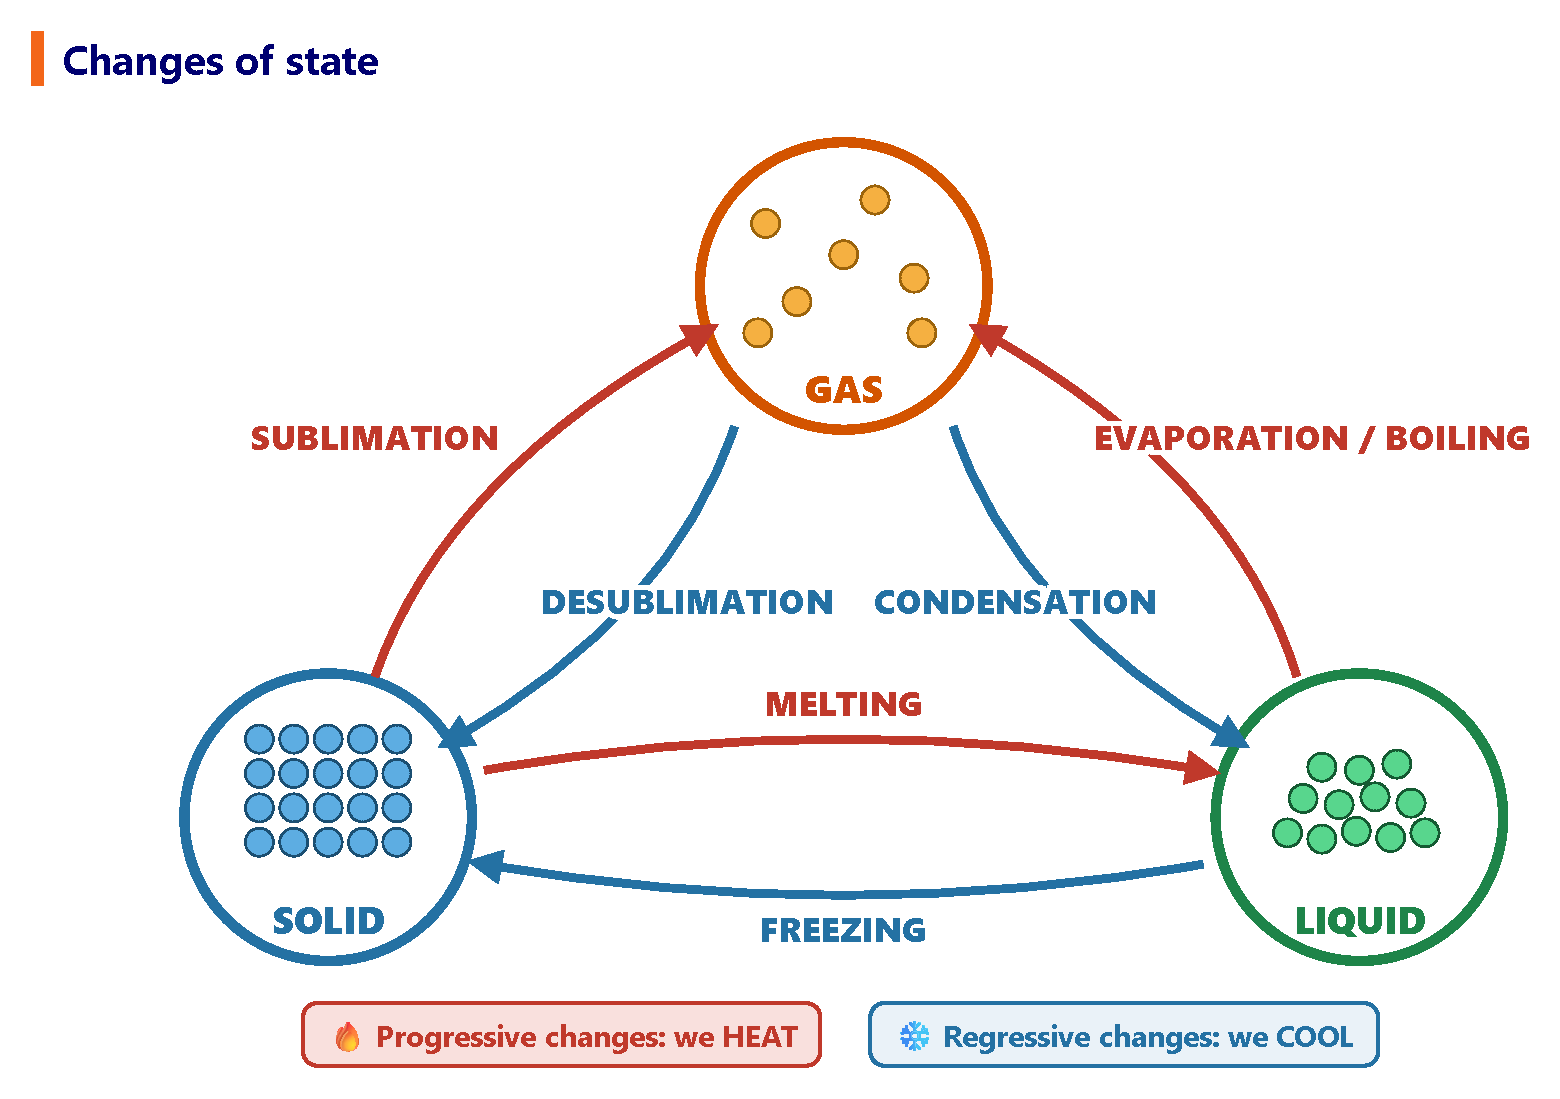
\includegraphics[width=0.95\textwidth]{FigurasSVG/Unit_2_State_of_Matter/pdf/changes_of_state.pdf}
    \caption{The six changes of state.}
    \label{fig:u2_changes_of_state}
\end{figure}

\begin{definition}[Melting point and boiling point]
    The \textbf{melting point} is the temperature at which a pure substance changes from solid to liquid; the \textbf{boiling point}, from liquid to gas. Both depend on pressure and are \textbf{characteristic properties}: each substance has its own values.
\end{definition}

\begin{table}[H]
    \centering
    \renewcommand{\arraystretch}{1.3}
    \begin{tabular}{lcc}
        \toprule
        \textbf{Substance} & \textbf{Melting point} & \textbf{Boiling point} \\
        \midrule
        Oxygen & \qty{-219}{\celsius} & \qty{-183}{\celsius} \\
        Alcohol & \qty{-114}{\celsius} & \qty{78}{\celsius} \\
        Mercury & \qty{-39}{\celsius} & \qty{357}{\celsius} \\
        Water & \qty{0}{\celsius} & \qty{100}{\celsius} \\
        Iron & \qty{1538}{\celsius} & \qty{2861}{\celsius} \\
        \bottomrule
    \end{tabular}
    \caption{Melting and boiling points of some substances.}
    \label{tab:u2_mp_bp}
\end{table}

\begin{impt}
    \textbf{Which state at room temperature?} Below its melting point a substance is \textbf{solid}; between its melting and boiling points it is \textbf{liquid}; above its boiling point it is a \textbf{gas}.
\end{impt}

\subsection{Heating curves and latent heat}

If we heat ice at a constant rate and write down its temperature every minute, we get a \negsubro{heating curve}:

\begin{figure}[H]
    \centering
    % [FIGURA ORIGINAL] \includegraphics[width=\textwidth]{Unit_2/heating_curve}
    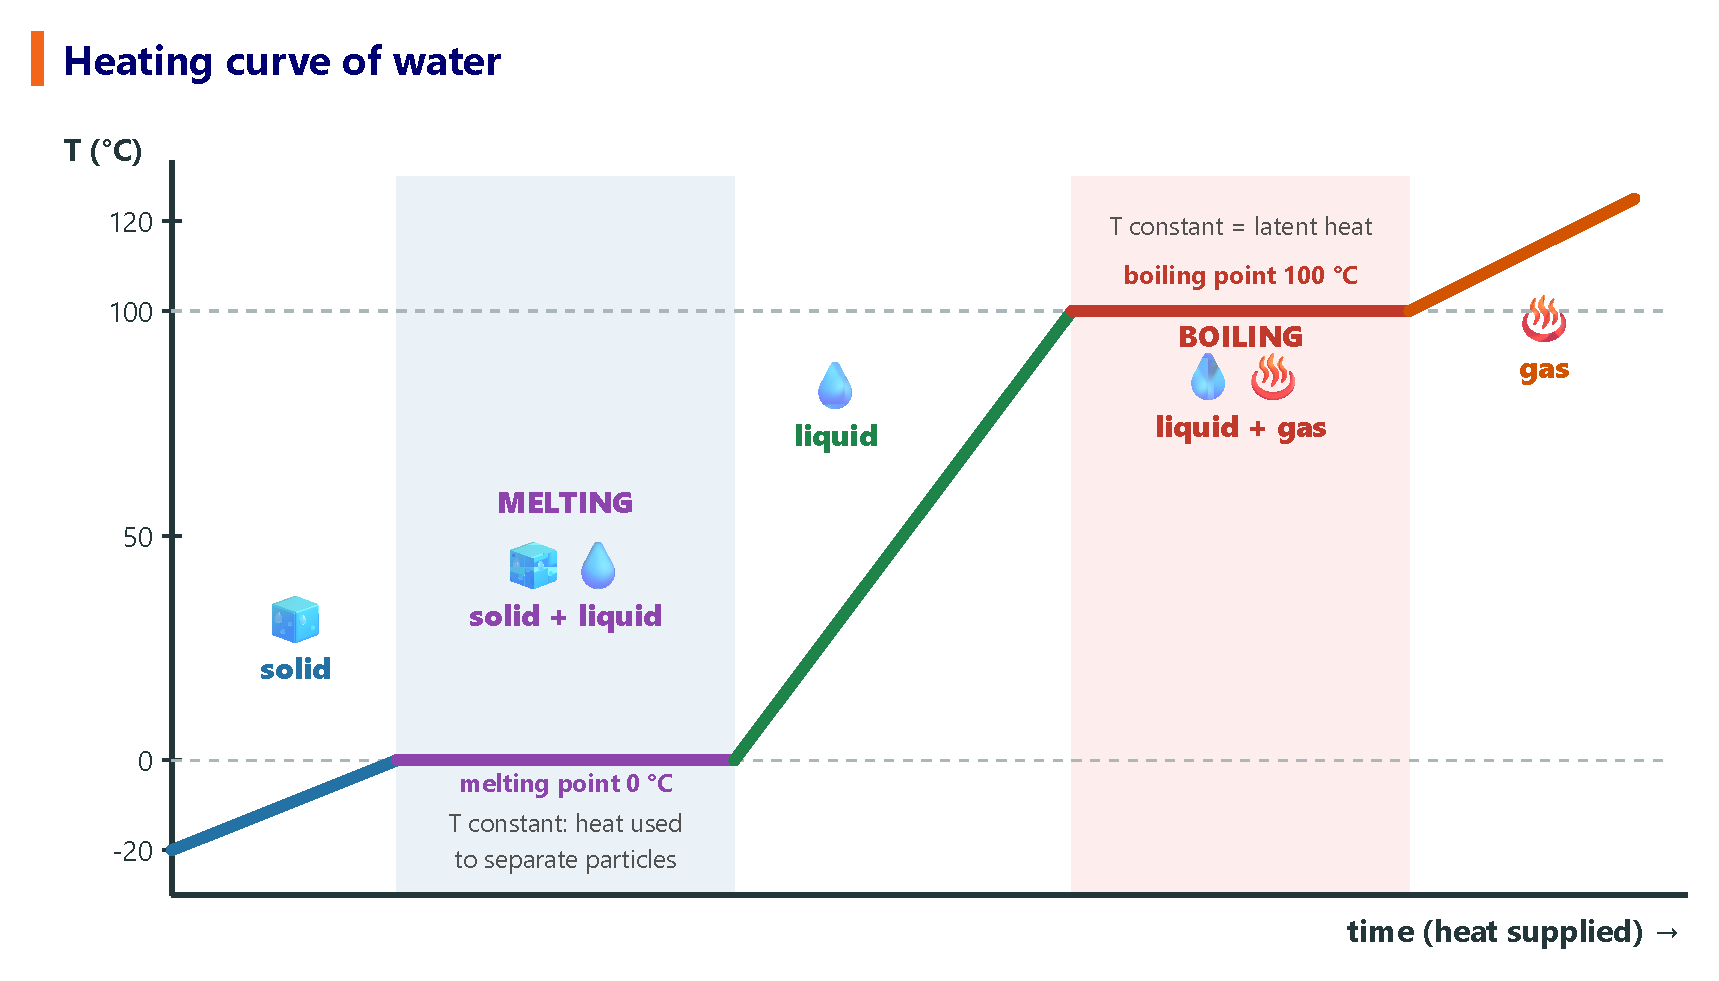
\includegraphics[width=\textwidth]{FigurasSVG/Unit_2_State_of_Matter/pdf/heating_curve.pdf}
    \caption{Heating curve of water: the temperature stays constant during each change of state.}
    \label{fig:u2_heating_curve}
\end{figure}

\begin{impt}
    While a pure substance is \textbf{changing state}, its \textbf{temperature does not change}, even if we keep heating it: the graph is flat (a ``plateau''). All the heat is used to separate the particles, not to make them move faster.
\end{impt}

\begin{definition}[Latent heat]
    The heat needed to change the state of \qty{1}{\kg} of a substance without changing its temperature. ``Latent'' means ``hidden'': we supply heat, but the thermometer does not show it.
\end{definition}

\subsection{Cooling curves}

If we do the opposite, and \textbf{cool} a substance at a constant rate while we write down its temperature every minute, we get a \negsubro{cooling curve}. It looks like the \textbf{mirror image} of the heating curve: the temperature goes \textbf{down}, and there are \textbf{plateaus} (flat parts) at the \textbf{same temperatures} as in the heating curve, while the gas condenses and while the liquid freezes.

\begin{figure}[H]
    \centering
    % [FIGURA ORIGINAL] \includegraphics[width=\textwidth]{Unit_2/cooling_curve}
    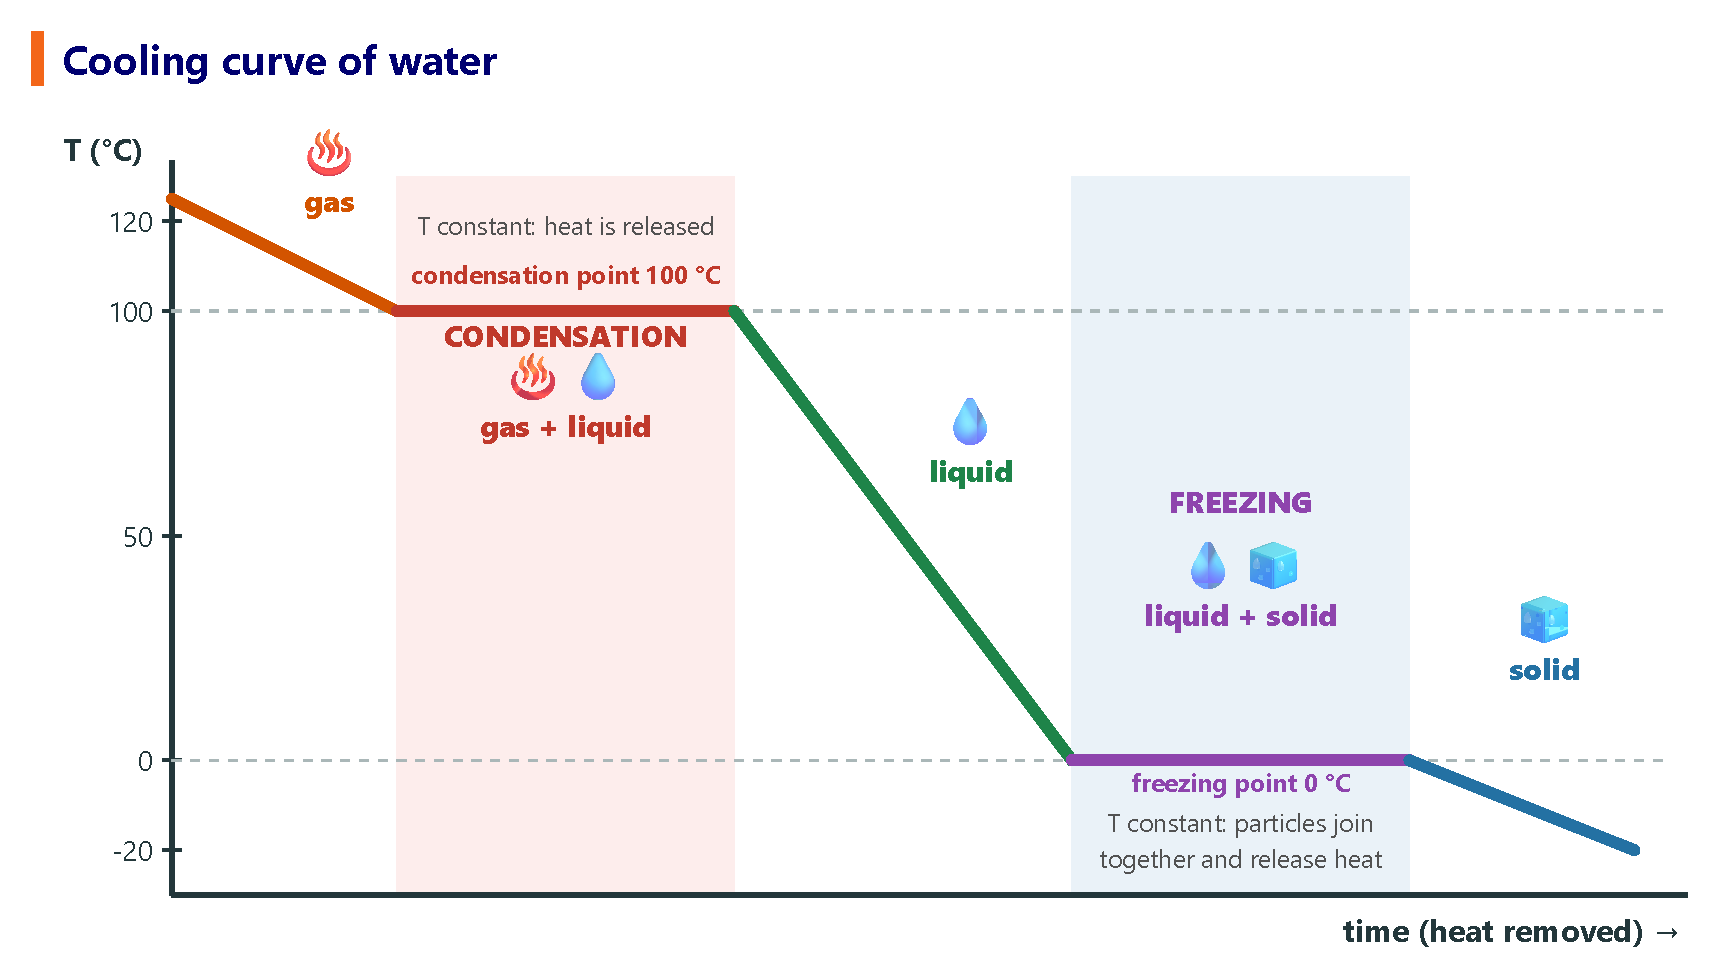
\includegraphics[width=\textwidth]{FigurasSVG/Unit_2_State_of_Matter/pdf/cooling_curve.pdf}
    \caption{Cooling curve of water: the temperature stays constant while the vapour condenses (\qty{100}{\celsius}) and while the liquid freezes (\qty{0}{\celsius}).}
    \label{fig:u2_cooling_curve}
\end{figure}

\begin{impt}
    \begin{itemize}
        \item In a cooling curve the substance \textbf{loses} heat. On the sloping parts its temperature goes down; on the flat parts it is \textbf{changing state} (condensation or freezing) and the temperature does \textbf{not} change.
        \item A pure substance \textbf{condenses} at the same temperature at which it \textbf{boils}, and it \textbf{freezes} at the same temperature at which it \textbf{melts}. For water: \qty{100}{\celsius} and \qty{0}{\celsius}.
    \end{itemize}
\end{impt}

\begin{example}
    \textbf{Reading the cooling curve of water.} We start with water vapour at \qty{125}{\celsius} and take heat away from it:
    \begin{enumerate}[label=\numberballmDarkTeal]
        \item From \qty{125}{\celsius} to \qty{100}{\celsius}: there is only \textbf{gas}, and its temperature goes down.
        \item At \qty{100}{\celsius}: the line is flat. The vapour is \textbf{condensing}: \textbf{gas and liquid} are together and the temperature does not change.
        \item From \qty{100}{\celsius} to \qty{0}{\celsius}: there is only \textbf{liquid}, and it gets colder.
        \item At \qty{0}{\celsius}: the line is flat again. The water is \textbf{freezing}: \textbf{liquid and solid} are together.
        \item Below \qty{0}{\celsius}: there is only \textbf{solid} (ice), and it keeps getting colder.
    \end{enumerate}
\end{example}

\begin{example}
    \textbf{Cooling curve of paraffin wax.} Liquid wax at \qty{80}{\celsius} is left to cool, and its temperature is written down every minute:
    \begin{center}
        \renewcommand{\arraystretch}{1.3}
        % --- tabla antigua ---
        % \begin{tabular}{l|cccccccc}
            % \textbf{Time (min)} & 0 & 1 & 2 & 3 & 4 & 5 & 6 & 7 \\
            % \hline
            % \textbf{T (\unit{\celsius})} & 80 & 70 & 60 & 55 & 55 & 55 & 45 & 35 \\
        % \end{tabular}
        % --- tabla nueva ---
        \begin{tabular}{@{}lcccccccc@{}}
            \toprule
            \textbf{Time (min)} & \textbf{0} & \textbf{1} & \textbf{2} & \textbf{3} & \textbf{4} & \textbf{5} & \textbf{6} & \textbf{7} \\
            \midrule
            \textbf{T (\unit{\celsius})} & 80 & 70 & 60 & 55 & 55 & 55 & 45 & 35 \\
            \bottomrule
        \end{tabular}
    \end{center}
    From minute 3 to minute 5 the temperature stays at \qty{55}{\celsius}: that is the plateau. So the wax \textbf{freezes} (and also melts) at \textcolor{red}{\qty{55}{\celsius}}. Before minute 3 the wax is liquid, between minutes 3 and 5 liquid and solid wax are together, and after minute 5 it is solid.
\end{example}

\begin{example}
    \textbf{Worked example: reading a heating curve step by step.} In the laboratory we heat an unknown pure substance at a constant rate, starting at \qty{-130}{\celsius}, and write down its temperature every minute:
    \begin{center}
        \renewcommand{\arraystretch}{1.3}
        \begin{tabular}{@{}lcccccccccccc@{}}
            \toprule
            \textbf{Time (min)} & \textbf{0} & \textbf{1} & \textbf{2} & \textbf{3} & \textbf{4} & \textbf{5} & \textbf{6} & \textbf{7} & \textbf{8} & \textbf{9} & \textbf{10} & \textbf{11} \\
            \midrule
            \textbf{T (\unit{\celsius})} & \(-130\) & \(-114\) & \(-114\) & \(-114\) & \(-50\) & 14 & 78 & 78 & 78 & 78 & 90 & 102 \\
            \bottomrule
        \end{tabular}
    \end{center}
    We want to know: \textbf{a)} its melting point and boiling point; \textbf{b)} its physical state in each part of the experiment; \textbf{c)} which substance it is.
    \begin{enumerate}[label=\numberballmDarkTeal]
        \item \textbf{Draw the graph.} Put the \textbf{time} on the horizontal axis and the \textbf{temperature} on the vertical axis, choose a scale that fits all the values (from \qty{-140}{\celsius} to \qty{120}{\celsius}), plot each pair of values as a point and join the points with straight lines (Figure~\ref{fig:u2_heating_curve_example}).
        \item \textbf{Look for the plateaus.} We look for the parts of the table where the temperature \textbf{does not change}, although we keep heating:
        \begin{itemize}
            \item from minute 1 to minute 3 the temperature stays at \qty{-114}{\celsius};
            \item from minute 6 to minute 9 the temperature stays at \qty{78}{\celsius}.
        \end{itemize}
        \item \textbf{Name the changes of state.} We are \textbf{heating}, so the first plateau (the lower temperature) is \textbf{melting} and the second one (the higher temperature) is \textbf{boiling}. Therefore:
        \[
            \text{melting point} = \textcolor{red}{\qty{-114}{\celsius}} \qquad \text{boiling point} = \textcolor{red}{\qty{78}{\celsius}}
        \]
        \item \textbf{Write the state in each part.} Below the melting point the substance is solid; on a plateau two states are together; between the two plateaus it is liquid; above the boiling point it is gas:
        \begin{itemize}
            \item from 0 to 1 min: \textbf{solid}, and its temperature goes up;
            \item from 1 to 3 min: \textbf{solid + liquid} (it is melting), constant temperature;
            \item from 3 to 6 min: \textbf{liquid}, and its temperature goes up;
            \item from 6 to 9 min: \textbf{liquid + gas} (it is boiling), constant temperature;
            \item from 9 to 11 min: \textbf{gas}, and its temperature goes up.
        \end{itemize}
        \item \textbf{Identify the substance.} Melting and boiling points are \textbf{characteristic properties}, so we compare our values with Table~\ref{tab:u2_mp_bp}: the substance that melts at \qty{-114}{\celsius} and boils at \qty{78}{\celsius} is \textcolor{red}{\textbf{alcohol}}.
        \item \textbf{Check the answer.} At room temperature (\qty{20}{\celsius}) our substance would be between its melting and boiling points, so it would be a \textbf{liquid}. That is right: alcohol is a liquid at room temperature.
    \end{enumerate}
\end{example}

\begin{figure}[H]
    \centering
    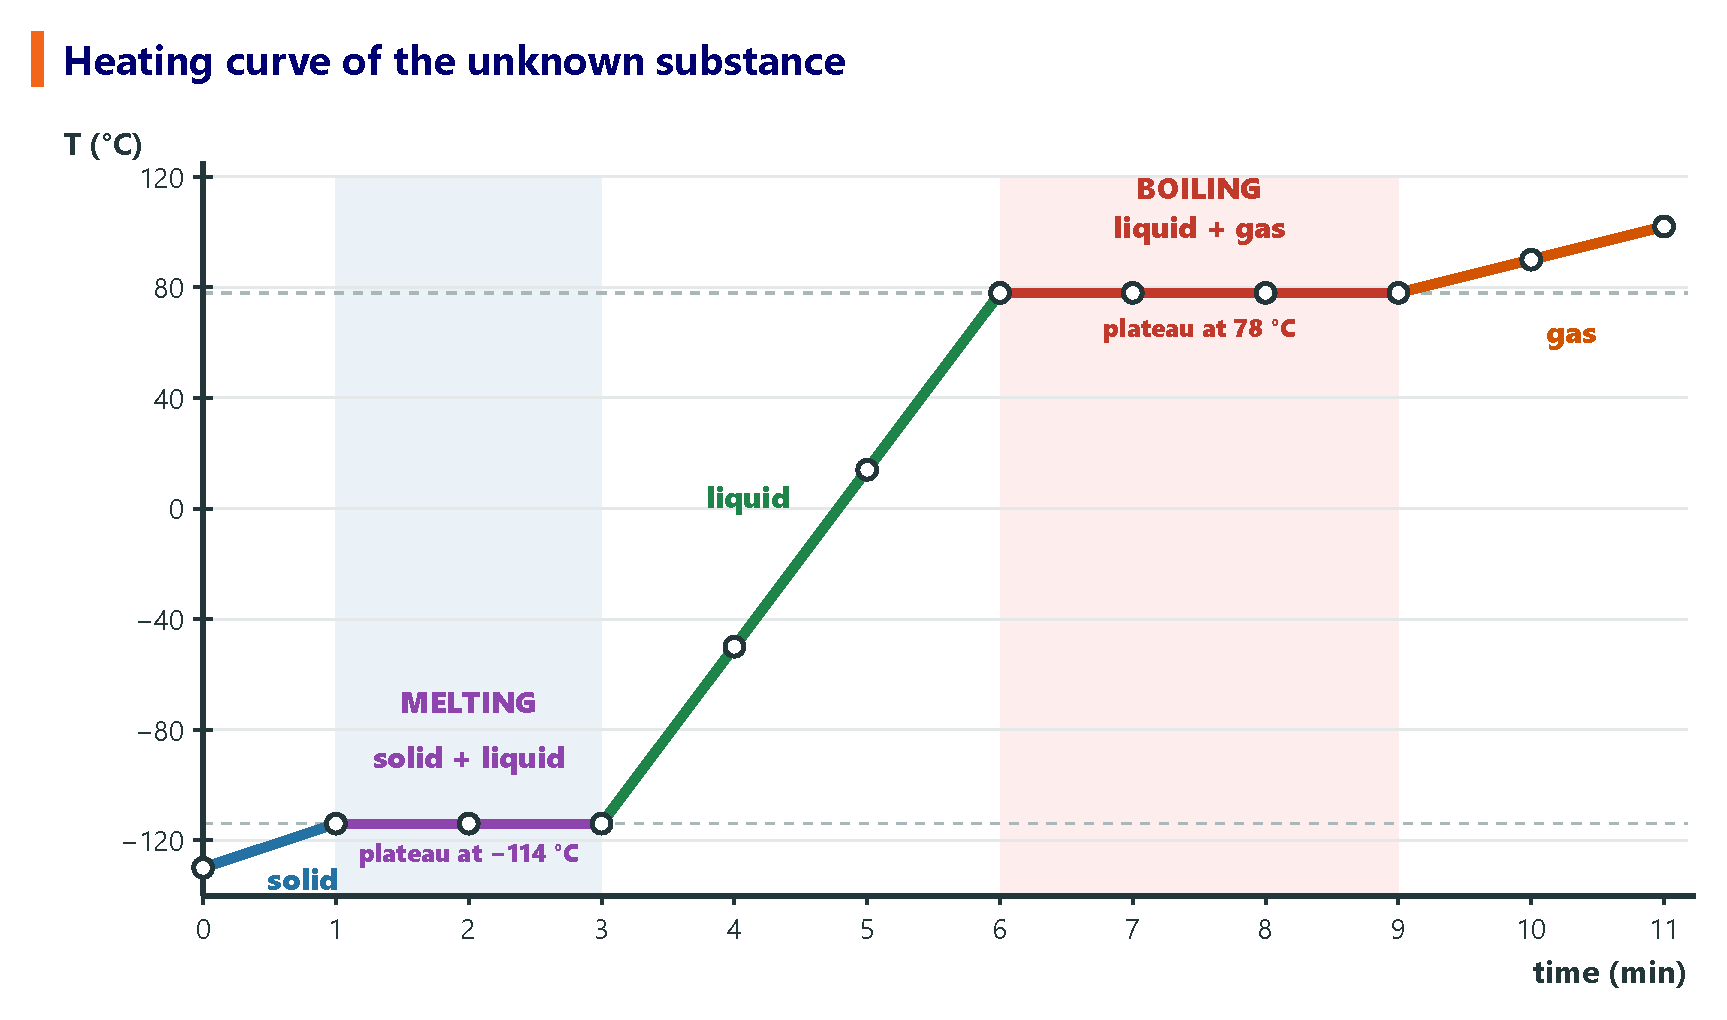
\includegraphics[width=\textwidth]{FigurasSVG/Unit_2_State_of_Matter/pdf/heating_curve_example.pdf}
    \caption{Heating curve drawn from the data of the worked example: the plateaus at \qty{-114}{\celsius} and \qty{78}{\celsius} are the melting and boiling points of alcohol.}
    \label{fig:u2_heating_curve_example}
\end{figure}

\begin{exercise}
    A sample of a pure substance is heated at a constant rate, and its temperature is recorded every minute: \qty{-10}{\celsius}, \qty{0}{\celsius}, \qty{0}{\celsius}, \qty{0}{\celsius}, \qty{20}{\celsius}, \qty{40}{\celsius} (at \(t = 0, 1, 2, 3, 4, 5\) min).
    \begin{enumerate}[label=\letraminuscula]
        \item What is the melting point of the substance?
        \item In which minutes is the substance changing state? Which states coexist?
        \item Could this substance be water? Justify your answer.
    \end{enumerate}
    \begin{solu}
        \begin{enumerate}[label=\alph*)]
            \item The temperature stays constant at \qty{0}{\celsius}, so the melting point is \qty{0}{\celsius}.
            \item Between \(t = 1\) and \(t = 3\) min; \textbf{solid and liquid} coexist.
            \item \textbf{Yes}, it could be water: its melting point (\qty{0}{\celsius}) matches the melting point of water at \qty{1}{\atmospher}.
        \end{enumerate}
    \end{solu}
\end{exercise}

\begin{exercise}
    Molten candle wax cools at room temperature, and its temperature is recorded every 2 minutes: \qty{80}{\celsius}, \qty{60}{\celsius}, \qty{45}{\celsius}, \qty{45}{\celsius}, \qty{45}{\celsius}, \qty{45}{\celsius}, \qty{30}{\celsius}, \qty{22}{\celsius} (at \(t = 0, 2, 4, 6, 8, 10, 12, 14\) min).
    \begin{enumerate}[label=\letraminuscula]
        \item Draw the cooling curve (temperature on the vertical axis, time on the horizontal axis).
        \item What is the freezing point of the wax?
        \item During which minutes is the wax changing state, and what states coexist?
    \end{enumerate}
    \begin{solu}
        \begin{enumerate}[label=\alph*)]
            \item The curve falls from \qty{80}{\celsius} to \qty{45}{\celsius}, stays flat at \qty{45}{\celsius} for several minutes, and then falls again to \qty{22}{\celsius}.
            \item \qty{45}{\celsius}.
            \item Between \(t = 4\) and \(t = 10\) min; \textbf{liquid and solid} wax coexist.
        \end{enumerate}
    \end{solu}
\end{exercise}

\begin{exercise}
    A student says: ``If I turn the gas on the stove up as high as possible, the water in the pan will boil at a much higher temperature, so my pasta will cook faster.'' Is the student right? Use the idea of latent heat.
    \begin{solu}
        The student is \textbf{wrong}. Once water reaches its boiling point (\qty{100}{\celsius} at \qty{1}{\atmospher}), its temperature stays constant however much heat we supply. More heat only makes the water boil \textbf{more vigorously}: the extra heat is used as latent heat to turn more liquid into gas, not to raise the temperature.
    \end{solu}
\end{exercise}

\subsection{Evaporation vs.\ boiling}

\begin{figure}[H]
    \centering
    % [FIGURA ORIGINAL] \includegraphics[width=\textwidth]{Unit_2/evaporation_boiling}
    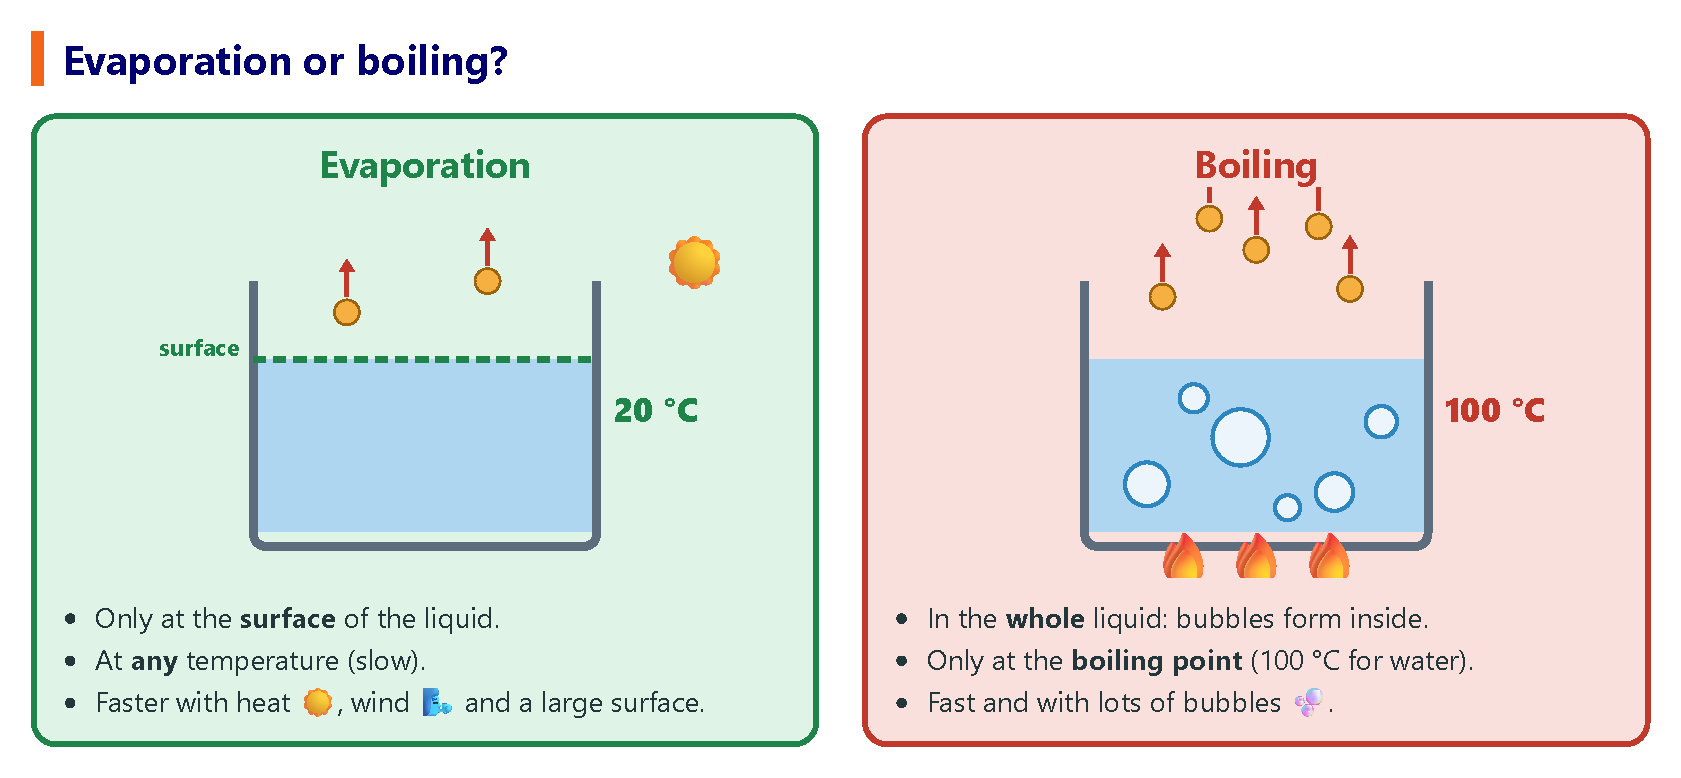
\includegraphics[width=\textwidth]{FigurasSVG/Unit_2_State_of_Matter/pdf/evaporation_boiling.pdf}
    \caption{Two ways of turning a liquid into a gas.}
    \label{fig:u2_evaporation_boiling}
\end{figure}

\begin{exercise}
    Classify each situation as evaporation or boiling, and justify your answer.
    \begin{enumerate}[label=\letraminuscula]
        \item Wet clothes hung out on a washing line dry after a few hours.
        \item Water in a saucepan bubbles vigorously on the stove at \qty{100}{\celsius}.
        \item A puddle on the pavement slowly disappears over a warm afternoon.
        \item Milk in a pan rises and bubbles all the way through just before it ``boils over''.
    \end{enumerate}
    \begin{solu}
        \begin{enumerate}[label=\alph*)]
            \item \textbf{Evaporation}: at the surface of the wet fabric, well below \qty{100}{\celsius}.
            \item \textbf{Boiling}: bubbles form throughout the whole liquid, at its boiling point.
            \item \textbf{Evaporation}: only at the surface of the puddle, at outdoor temperature.
            \item \textbf{Boiling}: the whole mass of milk is affected, not just the surface.
        \end{enumerate}
    \end{solu}
\end{exercise}

\begin{exercise}
    Explain why washing dries faster on a windy, sunny day than on a still, cloudy day, and why spreading the clothes out also makes them dry faster.
    \begin{solu}
        Drying clothes is \textbf{evaporation}. The Sun raises the temperature, so the water particles have more energy to escape; the wind carries the vapour away as soon as it forms. Spreading the clothes out increases the \textbf{surface area}, and evaporation is faster with a larger surface.
    \end{solu}
\end{exercise}

\subsection{Sublimation and desublimation}

Some substances, such as iodine or solid carbon dioxide (``dry ice''), change directly between solid and gas, \textbf{without} becoming a liquid:

\begin{itemize}
    \item \negsubro{Sublimation}: solid \(\to\) gas.
    \item \negsubro{Desublimation}: gas \(\to\) solid (for example, frost on a cold morning).
\end{itemize}

\begin{impt}
    Changes that happen when we \textbf{heat} (melting, evaporation, sublimation) are \negsubro{progressive}. Changes that happen when we \textbf{cool} (freezing, condensation, desublimation) are \negsubro{regressive}.
\end{impt}

\begin{didyouknow}
    The ``smoke'' that comes out of dry ice at concerts is not carbon dioxide gas, which is invisible! The very cold gas cools the air around it, and the water vapour in the air condenses into tiny drops: a man-made fog.
\end{didyouknow}

\begin{exercise}
    Blocks of solid carbon dioxide (``dry ice'') are often used to create a fog effect on stage.
    \begin{enumerate}[label=\letraminuscula]
        \item What change of state takes place as the dry ice ``disappears'', and is it progressive or regressive?
        \item Unlike an ice cube, dry ice never leaves a puddle of liquid behind. Why?
    \end{enumerate}
    \begin{solu}
        \begin{enumerate}[label=\alph*)]
            \item \textbf{Sublimation} (solid \(\to\) gas), a \textbf{progressive} change.
            \item At atmospheric pressure, solid carbon dioxide passes directly from solid to gas, without going through the liquid state.
        \end{enumerate}
    \end{solu}
\end{exercise}

\begin{exercise}
    Mothballs slowly get smaller over the weeks, even though they are never heated, and eventually disappear without leaving any liquid. Explain what is happening and name the change of state.
    \begin{solu}
        The mothball is \textbf{sublimating}: its particles pass directly from solid to gas (releasing a smell that repels insects), without ever becoming a liquid. This can happen slowly at room temperature.
    \end{solu}
\end{exercise}

\subsection{The effect of pressure on boiling}

\begin{figure}[H]
    \centering
    % [FIGURA ORIGINAL] \includegraphics[width=\textwidth]{Unit_2/pressure_boiling}
    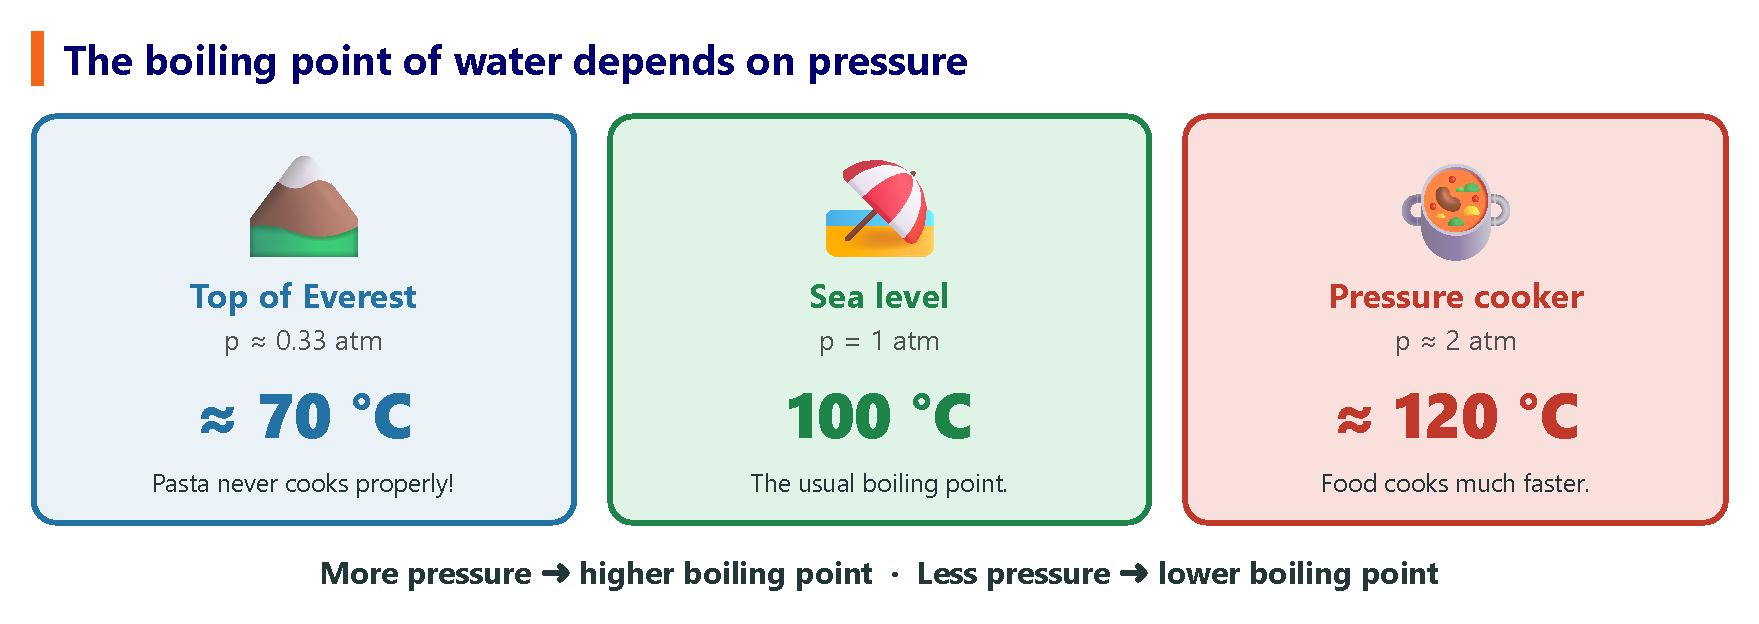
\includegraphics[width=\textwidth]{FigurasSVG/Unit_2_State_of_Matter/pdf/pressure_boiling.pdf}
    \caption{The boiling point of water changes with pressure.}
    \label{fig:u2_pressure_boiling}
\end{figure}

\begin{exercise}
    Use the table of melting and boiling points at the beginning of this section to indicate the physical state of oxygen, alcohol, water and iron at \qty{20}{\celsius} and \qty{1}{\atmospher}.
    \begin{solu}
        Oxygen: \textbf{gas} (\(20 > -183\)). \\
        Alcohol: \textbf{liquid} (\(-114 < 20 < 78\)). \\
        Water: \textbf{liquid} (\(0 < 20 < 100\)). \\
        Iron: \textbf{solid} (\(20 < 1538\)).
    \end{solu}
\end{exercise}

\begin{exercise}
    A liquid is cooled in a freezer. Its temperature is recorded every \qty{10}{\minute}: \qty{20}{\celsius}, \qty{6}{\celsius}, \qty{-8}{\celsius}, \qty{-8}{\celsius}, \qty{-8}{\celsius}, \qty{-22}{\celsius} (at \(t = 0, 10, 20, 30, 40, 50\) min).
    \begin{enumerate}[label=\letraminuscula]
        \item What is the freezing point of this substance?
        \item Can the substance be water? Why?
    \end{enumerate}
    \begin{solu}
        \begin{enumerate}[label=\alph*)]
            \item The temperature stays constant at \qty{-8}{\celsius} between \(t = 20\) and \(t = 40\) min, so the freezing point is \qty{-8}{\celsius}.
            \item \textbf{No}, because water freezes at \qty{0}{\celsius}.
        \end{enumerate}
    \end{solu}
\end{exercise}

\begin{exercise}
    A puddle dries up on a sunny day; the bathroom mirror steams up during a hot shower; frost forms on leaves on a very cold, clear night; an ice lolly drips in the sun. Identify the change of state in each case, and say whether it is progressive or regressive.
    \begin{solu}
        Puddle: \textbf{evaporation}, progressive. \\
        Mirror: \textbf{condensation}, regressive. \\
        Frost: \textbf{desublimation}, regressive. \\
        Ice lolly: \textbf{melting}, progressive.
    \end{solu}
\end{exercise}

%----------------------------------------------------------------------------------------

\section{States of water and meteorology}

Water is the only substance that we find naturally in the three states on Earth. Its changes of state create the weather we see every day:

\begin{figure}[H]
    \centering
    % [FIGURA ORIGINAL] \includegraphics[width=\textwidth]{Unit_2/weather_phenomena}
    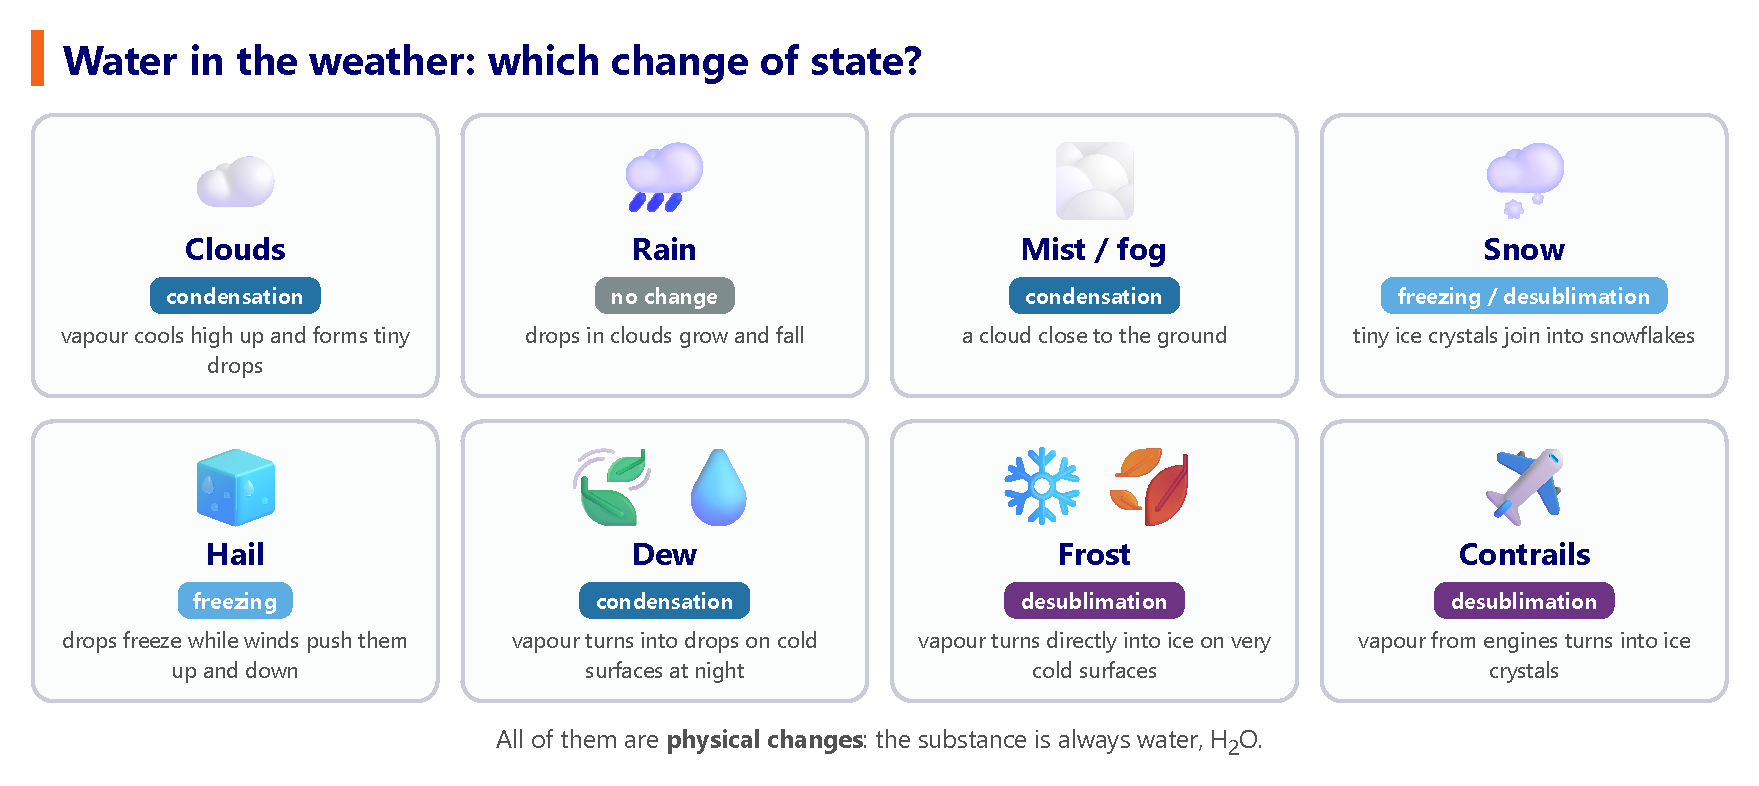
\includegraphics[width=\textwidth]{FigurasSVG/Unit_2_State_of_Matter/pdf/weather_phenomena.pdf}
    \caption{Weather phenomena and the change of state behind each one.}
    \label{fig:u2_weather_phenomena}
\end{figure}

\begin{exercise}
    Name the physical state in which water is found in: clouds, air, hail, snow, dew, frost.
    \begin{solu}
        Clouds: liquid (drops) or solid (ice crystals). Air: gas (water vapour). Hail: solid. Snow: solid. Dew: liquid. Frost: solid.
    \end{solu}
\end{exercise}

\begin{exercise}
    When we breathe out on a cold winter day, we can see a small cloud coming out of our mouths, but this does not happen indoors. Why?
    \begin{solu}
        Our breath contains warm water vapour. Outdoors, in cold air, it cools very quickly and \textbf{condenses} into tiny visible drops. Indoors, the air is warmer, so the vapour does not condense and stays as an invisible gas.
    \end{solu}
\end{exercise}

\begin{exercise}
    Match each weather phenomenon with the change of state involved, and say whether it is progressive or regressive: (1) dew, (2) frost, (3) mist, (4) hail.
    \begin{enumerate}[label=\letraminuscula]
        \item[A] Condensation of water vapour into liquid drops.
        \item[B] Desublimation of water vapour directly into a solid.
        \item[C] Evaporation followed by condensation close to the ground.
        \item[D] Freezing of liquid drops carried up and down inside a cloud.
    \end{enumerate}
    \begin{solu}
        (1) Dew \(\to\) A, condensation, regressive. \\
        (2) Frost \(\to\) B, desublimation, regressive. \\
        (3) Mist \(\to\) C, evaporation (progressive) followed by condensation (regressive); the visible mist itself is formed by condensation. \\
        (4) Hail \(\to\) D, freezing, regressive.
    \end{solu}
\end{exercise}

\subsection{The water cycle}

Water is always moving between the sea, the air and the land, and changing state on the way. This is the \negsubro{water cycle}, and its engine is the \textbf{Sun}.

\begin{figure}[H]
    \centering
    % [FIGURA ORIGINAL] \includegraphics[width=\textwidth]{Unit_2/water_cycle}
    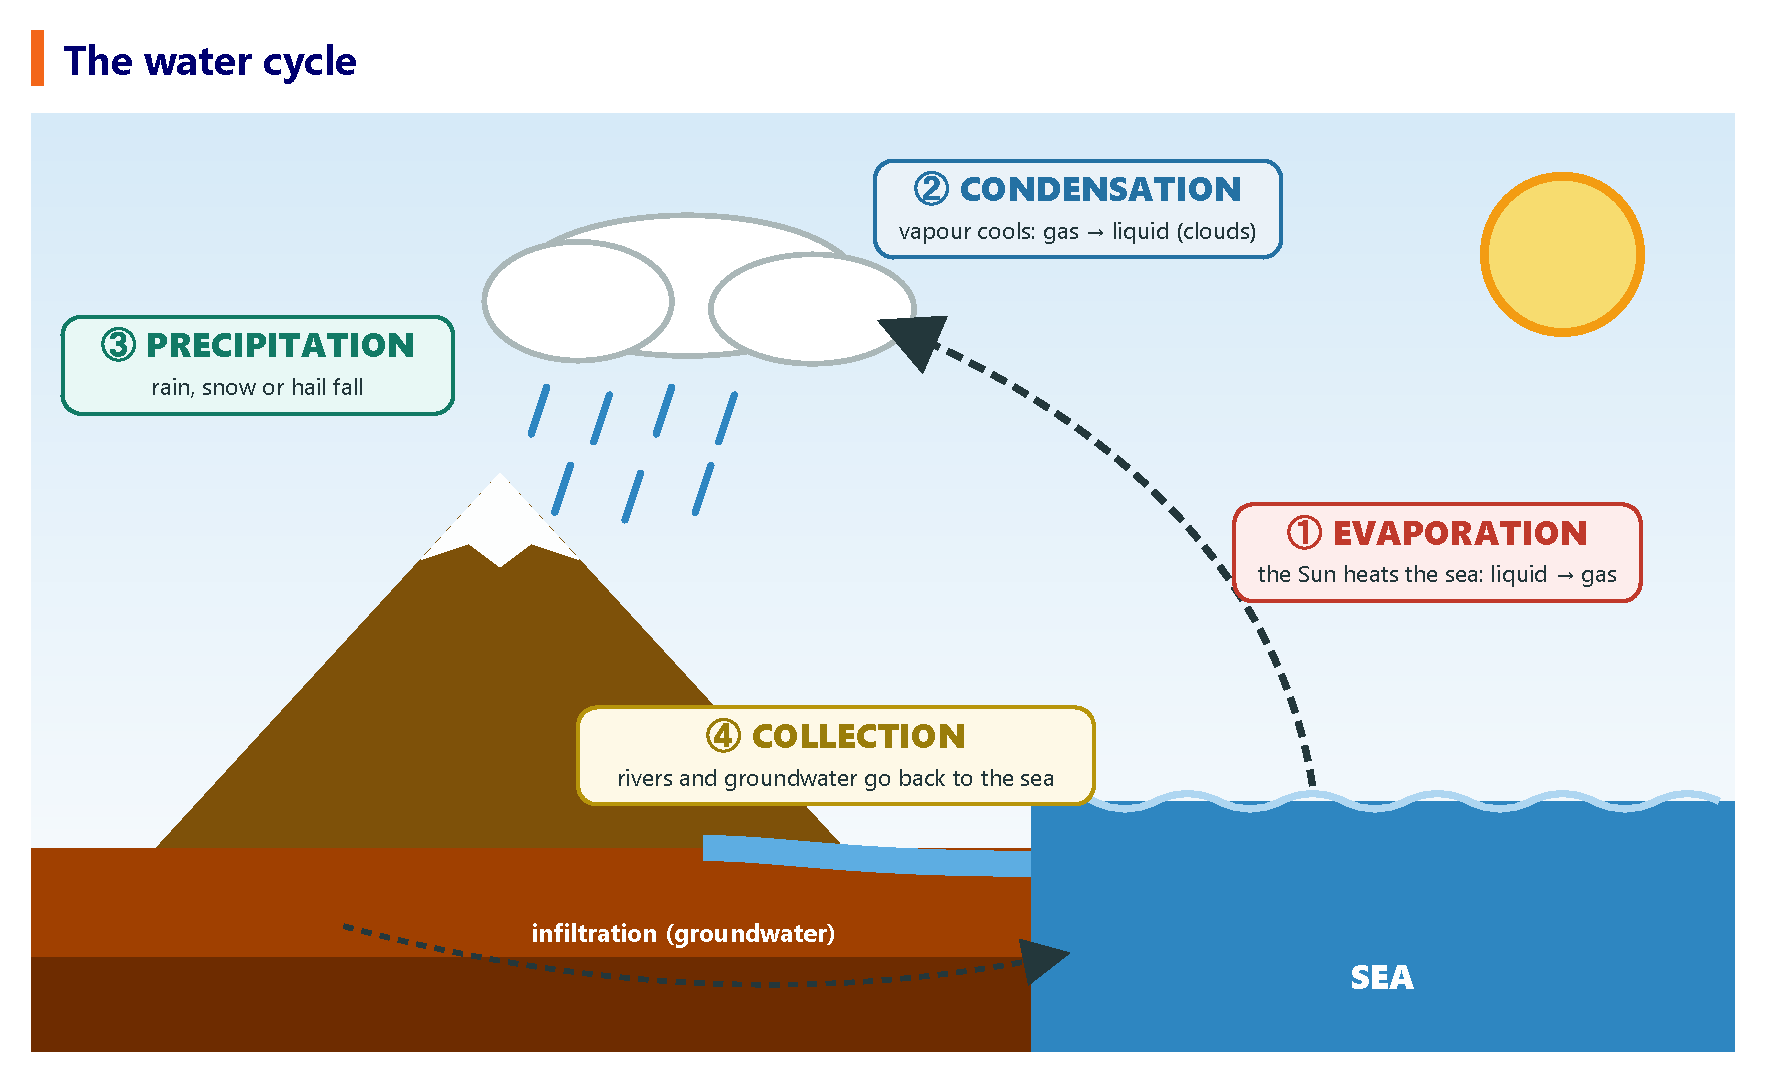
\includegraphics[width=\textwidth]{FigurasSVG/Unit_2_State_of_Matter/pdf/water_cycle.pdf}
    \caption{The four stages of the water cycle.}
    \label{fig:u2_water_cycle}
\end{figure}

\begin{impt}
    The water cycle involves \textbf{only physical changes}: the substance is always water, \ch{H2O}, whatever state it is in.
\end{impt}

\begin{didyouknow}
    The water you drink today is the same water the dinosaurs drank millions of years ago! The amount of water on Earth hardly changes: it just keeps going round and round the water cycle.
\end{didyouknow}

\begin{exercise}
    Order these stages of the water cycle correctly, and name the change of state involved in each one: (1) clouds form over the sea; (2) rain falls over the mountains; (3) the Sun heats the surface of the ocean; (4) rivers carry the water back to the sea.
    \begin{solu}
        Correct order: 3, 1, 2, 4. \\
        (3) Water turns into vapour: \textbf{evaporation}. \\
        (1) Water vapour cools down and forms tiny droplets: \textbf{condensation}. \\
        (2) The droplets grow and fall: \textbf{precipitation} (no change of state). \\
        (4) Liquid water flows back to the sea (no change of state).
    \end{solu}
\end{exercise}

\begin{exercise}
    Explain why the water cycle is said to involve ``only physical changes'', and why it could not continue without the Sun.
    \begin{solu}
        Although water changes state many times, it is always the \textbf{same substance}, \ch{H2O}: no new substances are formed. The Sun supplies the energy needed for \textbf{evaporation}; without it, no water vapour would form, there would be no clouds and no precipitation.
    \end{solu}
\end{exercise}

\begin{exercise}
    ``Most of the water that falls as rain over a mountain range originally evaporated from the ocean, sometimes hundreds of kilometres away.''
    \begin{enumerate}[label=\letraminuscula]
        \item Describe, step by step, how a water particle could travel from the ocean to a raindrop falling on a mountain.
        \item Once the rain falls on the mountain, name two possible paths the water can then follow.
    \end{enumerate}
    \begin{solu}
        \begin{enumerate}[label=\alph*)]
            \item The Sun heats the ocean and the water \textbf{evaporates}. Winds carry the vapour inland; as it rises over the mountains it cools and \textbf{condenses} into tiny droplets (a cloud). When the droplets are big enough they fall as \textbf{rain}.
            \item It can flow over the surface (streams and rivers) back to the sea, or \textbf{infiltrate} into the ground and become groundwater.
        \end{enumerate}
    \end{solu}
\end{exercise}

%----------------------------------------------------------------------------------------

\section*{Summary}

\begin{itemize}
    \item \textbf{States of matter}: solids (fixed shape and volume), liquids (fixed volume, variable shape), gases (variable shape and volume).
    \item \textbf{Kinetic theory}: matter is made of particles that are always moving; the faster they move, the higher the temperature. It explains diffusion, compressibility, thermal expansion and gas pressure.
    \item \textbf{Gas pressure}: caused by gas particles hitting the walls of the container.
    \item \textbf{Gas laws} (temperature always in kelvin, \(T(\unit{\K}) = T(\unit{\celsius}) + 273\)): Boyle-Mariotte (\(p \cdot V = \text{const.}\)); Gay-Lussac (\(p/T = \text{const.}\)); Charles (\(V/T = \text{const.}\)); general gas law (\(p \cdot V / T = \text{const.}\)).
    \item \textbf{Changes of state}: progressive (melting, evaporation/boiling, sublimation) and regressive (freezing, condensation, desublimation). The temperature stays constant during a change of state, because the heat is used as \textbf{latent heat}.
    \item \textbf{Evaporation} happens at the surface, at any temperature; \textbf{boiling} happens in the whole liquid, at the boiling point.
    \item \textbf{Pressure and boiling point}: more pressure \(\to\) higher boiling point (pressure cooker); less pressure \(\to\) lower boiling point (mountains).
    \item \textbf{Meteorology and the water cycle}: clouds, mist and dew form by condensation; frost and contrails by desublimation; hail by freezing. The Sun drives the water cycle: evaporation, condensation, precipitation and collection.
\end{itemize}

\section{Vocabulary}

\begin{vocabulary}[Kinetic theory]
    The theory explaining that matter is made up of moving particles, whose behaviour depends on their state. \newline
    \textbf{Translation to Spanish}: Teoría cinética
\end{vocabulary}

\begin{vocabulary}[Melting]
    Change of state from solid to liquid. \newline
    \textbf{Translation to Spanish}: Fusión
\end{vocabulary}

\begin{vocabulary}[Freezing]
    Change of state from liquid to solid. \newline
    \textbf{Translation to Spanish}: Solidificación
\end{vocabulary}

\begin{vocabulary}[Evaporation]
    Change of state from liquid to gas, occurring at the surface of the liquid. \newline
    \textbf{Translation to Spanish}: Evaporación
\end{vocabulary}

\begin{vocabulary}[Boiling]
    Change of state from liquid to gas, occurring throughout the liquid at the boiling point. \newline
    \textbf{Translation to Spanish}: Ebullición
\end{vocabulary}

\begin{vocabulary}[Condensation]
    Change of state from gas to liquid. \newline
    \textbf{Translation to Spanish}: Condensación
\end{vocabulary}

\begin{vocabulary}[Sublimation]
    Change of state directly from solid to gas. \newline
    \textbf{Translation to Spanish}: Sublimación
\end{vocabulary}

\begin{vocabulary}[Desublimation]
    Change of state directly from gas to solid. \newline
    \textbf{Translation to Spanish}: Sublimación inversa
\end{vocabulary}

\begin{vocabulary}[Melting point]
    Temperature at which a substance changes from solid to liquid. \newline
    \textbf{Translation to Spanish}: Punto de fusión
\end{vocabulary}

\begin{vocabulary}[Boiling point]
    Temperature at which a substance changes from liquid to gas. \newline
    \textbf{Translation to Spanish}: Punto de ebullición
\end{vocabulary}

\begin{vocabulary}[Pressure]
    The force exerted by the particles of a gas as they hit the walls of the container. \newline
    \textbf{Translation to Spanish}: Presión
\end{vocabulary}

\begin{vocabulary}[Diffusion]
    The process by which the particles of a gas or liquid spread out and mix, until they are evenly distributed. \newline
    \textbf{Translation to Spanish}: Difusión
\end{vocabulary}

\begin{vocabulary}[General gas law]
    The equation $p \cdot V / T = \text{constant}$, which relates pressure, volume and temperature when none of the three is fixed. \newline
    \textbf{Translation to Spanish}: Ley general de los gases
\end{vocabulary}

\begin{vocabulary}[Heating curve]
    A graph showing how the temperature of a substance changes over time as it is heated at a constant rate, with flat sections during changes of state. \newline
    \textbf{Translation to Spanish}: Curva de calentamiento
\end{vocabulary}

\begin{vocabulary}[Latent heat]
    The heat needed to change the state of a substance at constant temperature. \newline
    \textbf{Translation to Spanish}: Calor latente
\end{vocabulary}

\begin{vocabulary}[Absolute zero]
    The lowest possible temperature, 0 K (\qty{-273}{\celsius}), at which particles stop moving. \newline
    \textbf{Translation to Spanish}: Cero absoluto
\end{vocabulary}

\begin{vocabulary}[Progressive change]
    A change of state that happens when a substance is heated (melting, evaporation, sublimation). \newline
    \textbf{Translation to Spanish}: Cambio progresivo
\end{vocabulary}

\begin{vocabulary}[Regressive change]
    A change of state that happens when a substance is cooled (freezing, condensation, desublimation). \newline
    \textbf{Translation to Spanish}: Cambio regresivo
\end{vocabulary}

\begin{vocabulary}[Water cycle]
    The continuous movement of water between the oceans, the atmosphere and the land, through evaporation, condensation, precipitation and collection. \newline
    \textbf{Translation to Spanish}: Ciclo del agua
\end{vocabulary}
